\documentclass[letterpaper, 10 pt, conference]{article} 
\usepackage[english]{babel}
\usepackage{amsmath,amssymb,amscd,amsthm} % variety of useful math macros
\usepackage[inner=1.5 cm, outer = 1.5 cm, top=1 cm, bottom = 1.5 cm]{geometry}
\usepackage{subcaption}
%Para insertar imágenes
\usepackage{graphicx}
\usepackage[dvipsnames]{xcolor}
\usepackage{listings}
\usepackage[utf8]{inputenc}
\usepackage{hyperref}
%Para crear diagramas
%\usepackage{tikz} 

\newcommand\N{\ensuremath{\mathcal{N}}}

\title{A text analysis of Nietzsche's \it{Antichrist}}
\author{G. Palafox}

\lstset{ 
	basicstyle=\footnotesize,        % the size of the fonts that are used for the code
	breakatwhitespace=false,         % sets if automatic breaks should only happen at whitespace
	breaklines=true,                 % sets automatic line breaking
	showspaces=false,                % show spaces everywhere adding particular underscores; it overrides 
	showstringspaces = false,
	stringstyle=\color{MidnightBlue},     % string literal style
	backgroundcolor=\color{White},   
}

\begin{document}

\maketitle

\begin{abstract}
	In the following report, we show the results of employing basic text analysis techniques on Friedrich Nietzsche's book \emph{The Antichrist}. Graphics are shown to aid with the exposition of our findings.
\end{abstract}

\section{Introduction}
A text analysis of Nietzsche's \textit{The Antichrist} \cite{antichrist} was done. We were able to find the most common words and characters in the text, omitting numbers and really common words (e.g., \textquotedblleft the\textquotedblright). We used these words and characters to create various barplots and a word cloud visualization. Furthermore, we determined the most common pairs of words occurring together in the text, and show them with a network representation of our book.

\section{Text Analysis}
The text extraction and analysis was performed in a Jupyter\cite{jupyter} notebook running R\cite{R} version 4.0.0\footnote{The script and a Jupyter \cite{jupyter} notebook showing how we performed the data analysis and created the graphics in this report can be found at \url{https://github.com/palafox794/AppliedProbabilityModels/tree/master/Assignment2}}. We downloaded the book directly from Project Gutenberg's site using R's \texttt{gutenbergr} library. The book downloaded starts with an introduction by the translator, which we ommitted from the analysis, as the intention was to study the author's words.
Our first step into analysing the text was to get the most frequent characters and words. For this we ommitted numbers, punctuaction, and so-called stop-words. Table \ref{tab:words-chars} shows the ten most used letters and ten most used words in the text. Additionally, frequency of characters and words are shown in the barplots of Figure \ref{fig:barplots_chars_words}. For illustration purposes, we show a word cloud of the most frequent words in Figure \ref{fig:wordcloud}. In a word cloud, the size of each word is proportional to the number of times it appears in the text.

\begin{table}[ht]
\caption{Word and character frequency}
\begin{subtable}[ht]{0.45\textwidth}
\centering
\caption{Character frequency}
\begin{tabular}{rlr}
  \hline
 & Letter & Frequency \\ 
  \hline
1 & e & 15765 \\ 
  2 & t & 12898 \\ 
  3 & i & 10155 \\ 
  4 & a & 10052 \\ 
  5 & o & 9902 \\ 
  6 & s & 9114 \\ 
  7 & n & 9040 \\ 
  8 & h & 7654 \\ 
  9 & r & 7061 \\ 
  10 & l & 5291 \\ 
   \hline
\end{tabular}
\end{subtable}
\hfill
\begin{subtable}[ht]{0.45\textwidth}
\centering
\caption{Word frequency}
\begin{tabular}{rlr}
  \hline
 & Word & Frequency \\ 
  \hline
1 & god & 172 \\ 
  2 & life &  96 \\ 
  3 & christian &  90 \\ 
  4 & christianity &  89 \\ 
  5 & world &  78 \\ 
  6 & truth &  54 \\ 
  7 & priest &  49 \\ 
  8 & sort &  48 \\ 
  9 & instinct &  47 \\ 
  10 & power &  46 \\ 
   \hline
\end{tabular}
\end{subtable}
\label{tab:words-chars}
\end{table}

 \begin{figure}
 	\centering
 	\caption{Barplots of words and characters occurences.} 
 	\begin{subfigure}[b]{0.45\linewidth}
 		\caption{Character occurrence.}
 		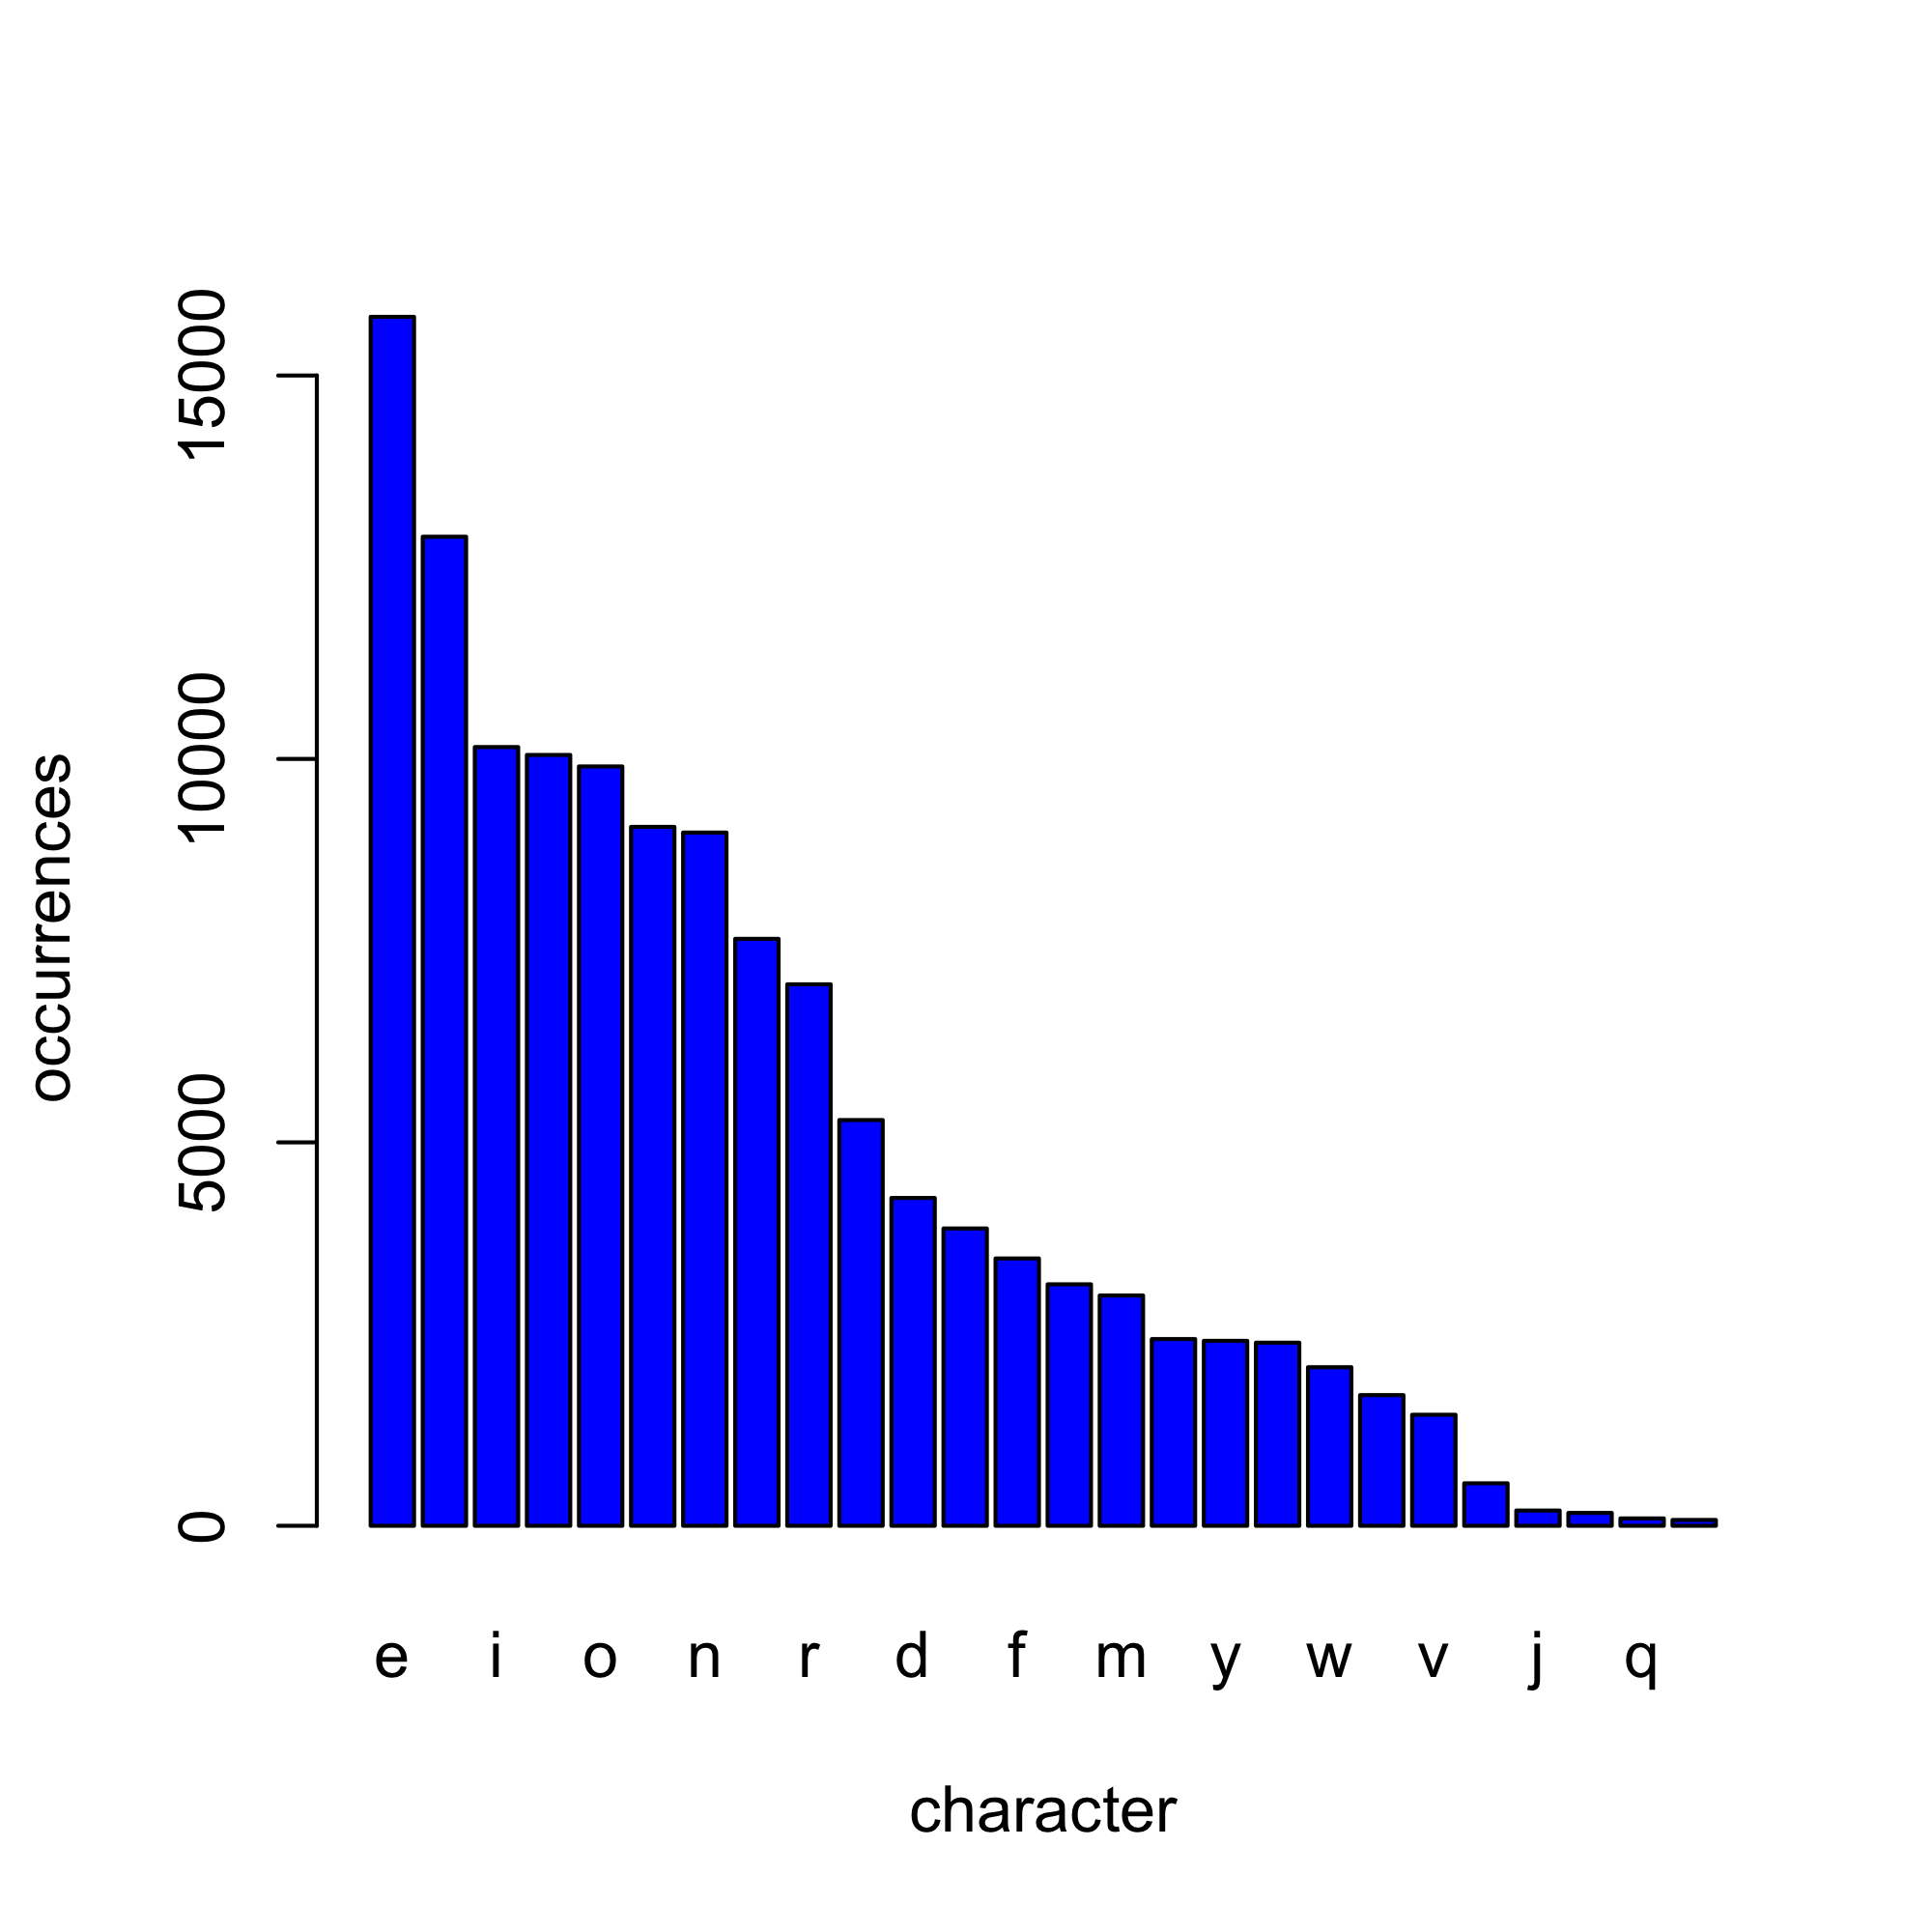
\includegraphics[width=\linewidth]{barplot_characters.png}
 	\end{subfigure}
 	\begin{subfigure}[b]{0.45\linewidth}
 		\caption{Most-frequent character occurrence.}
 		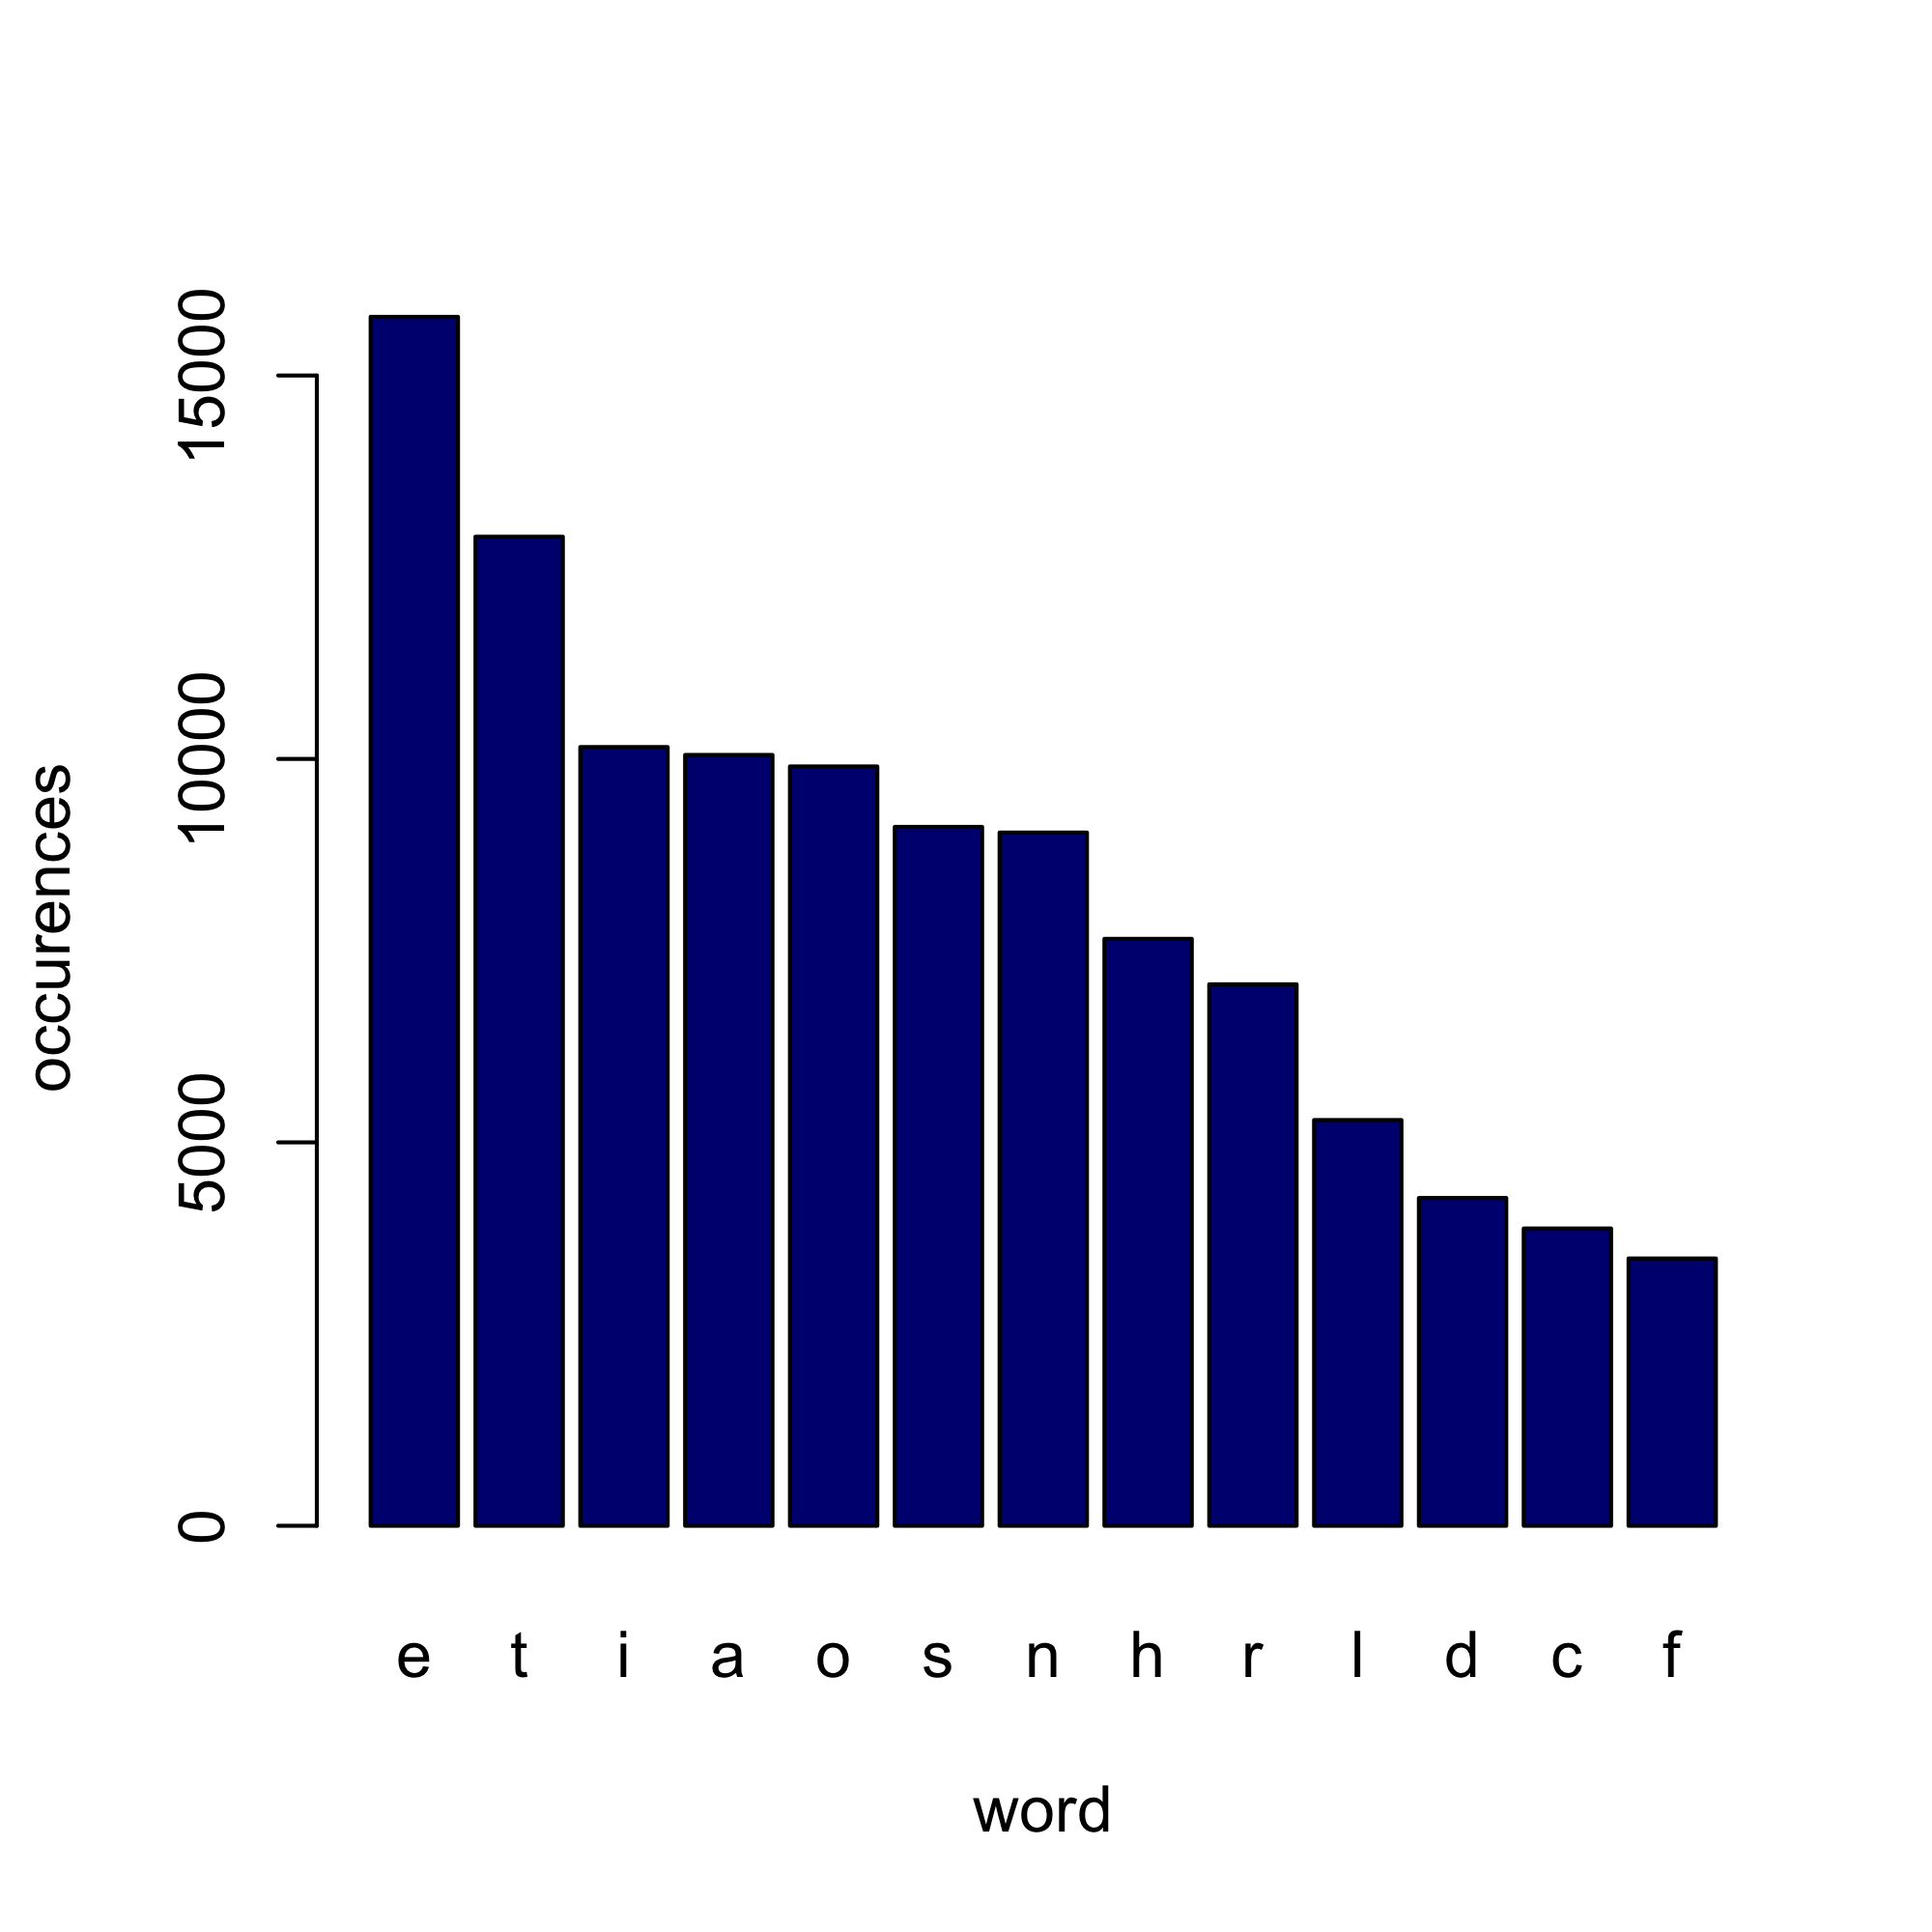
\includegraphics[width=\linewidth]{barplot_freq_chars.png}
 	\end{subfigure}
 	\begin{subfigure}[b]{0.45\linewidth}
 		\caption{Word occurrence.}
 		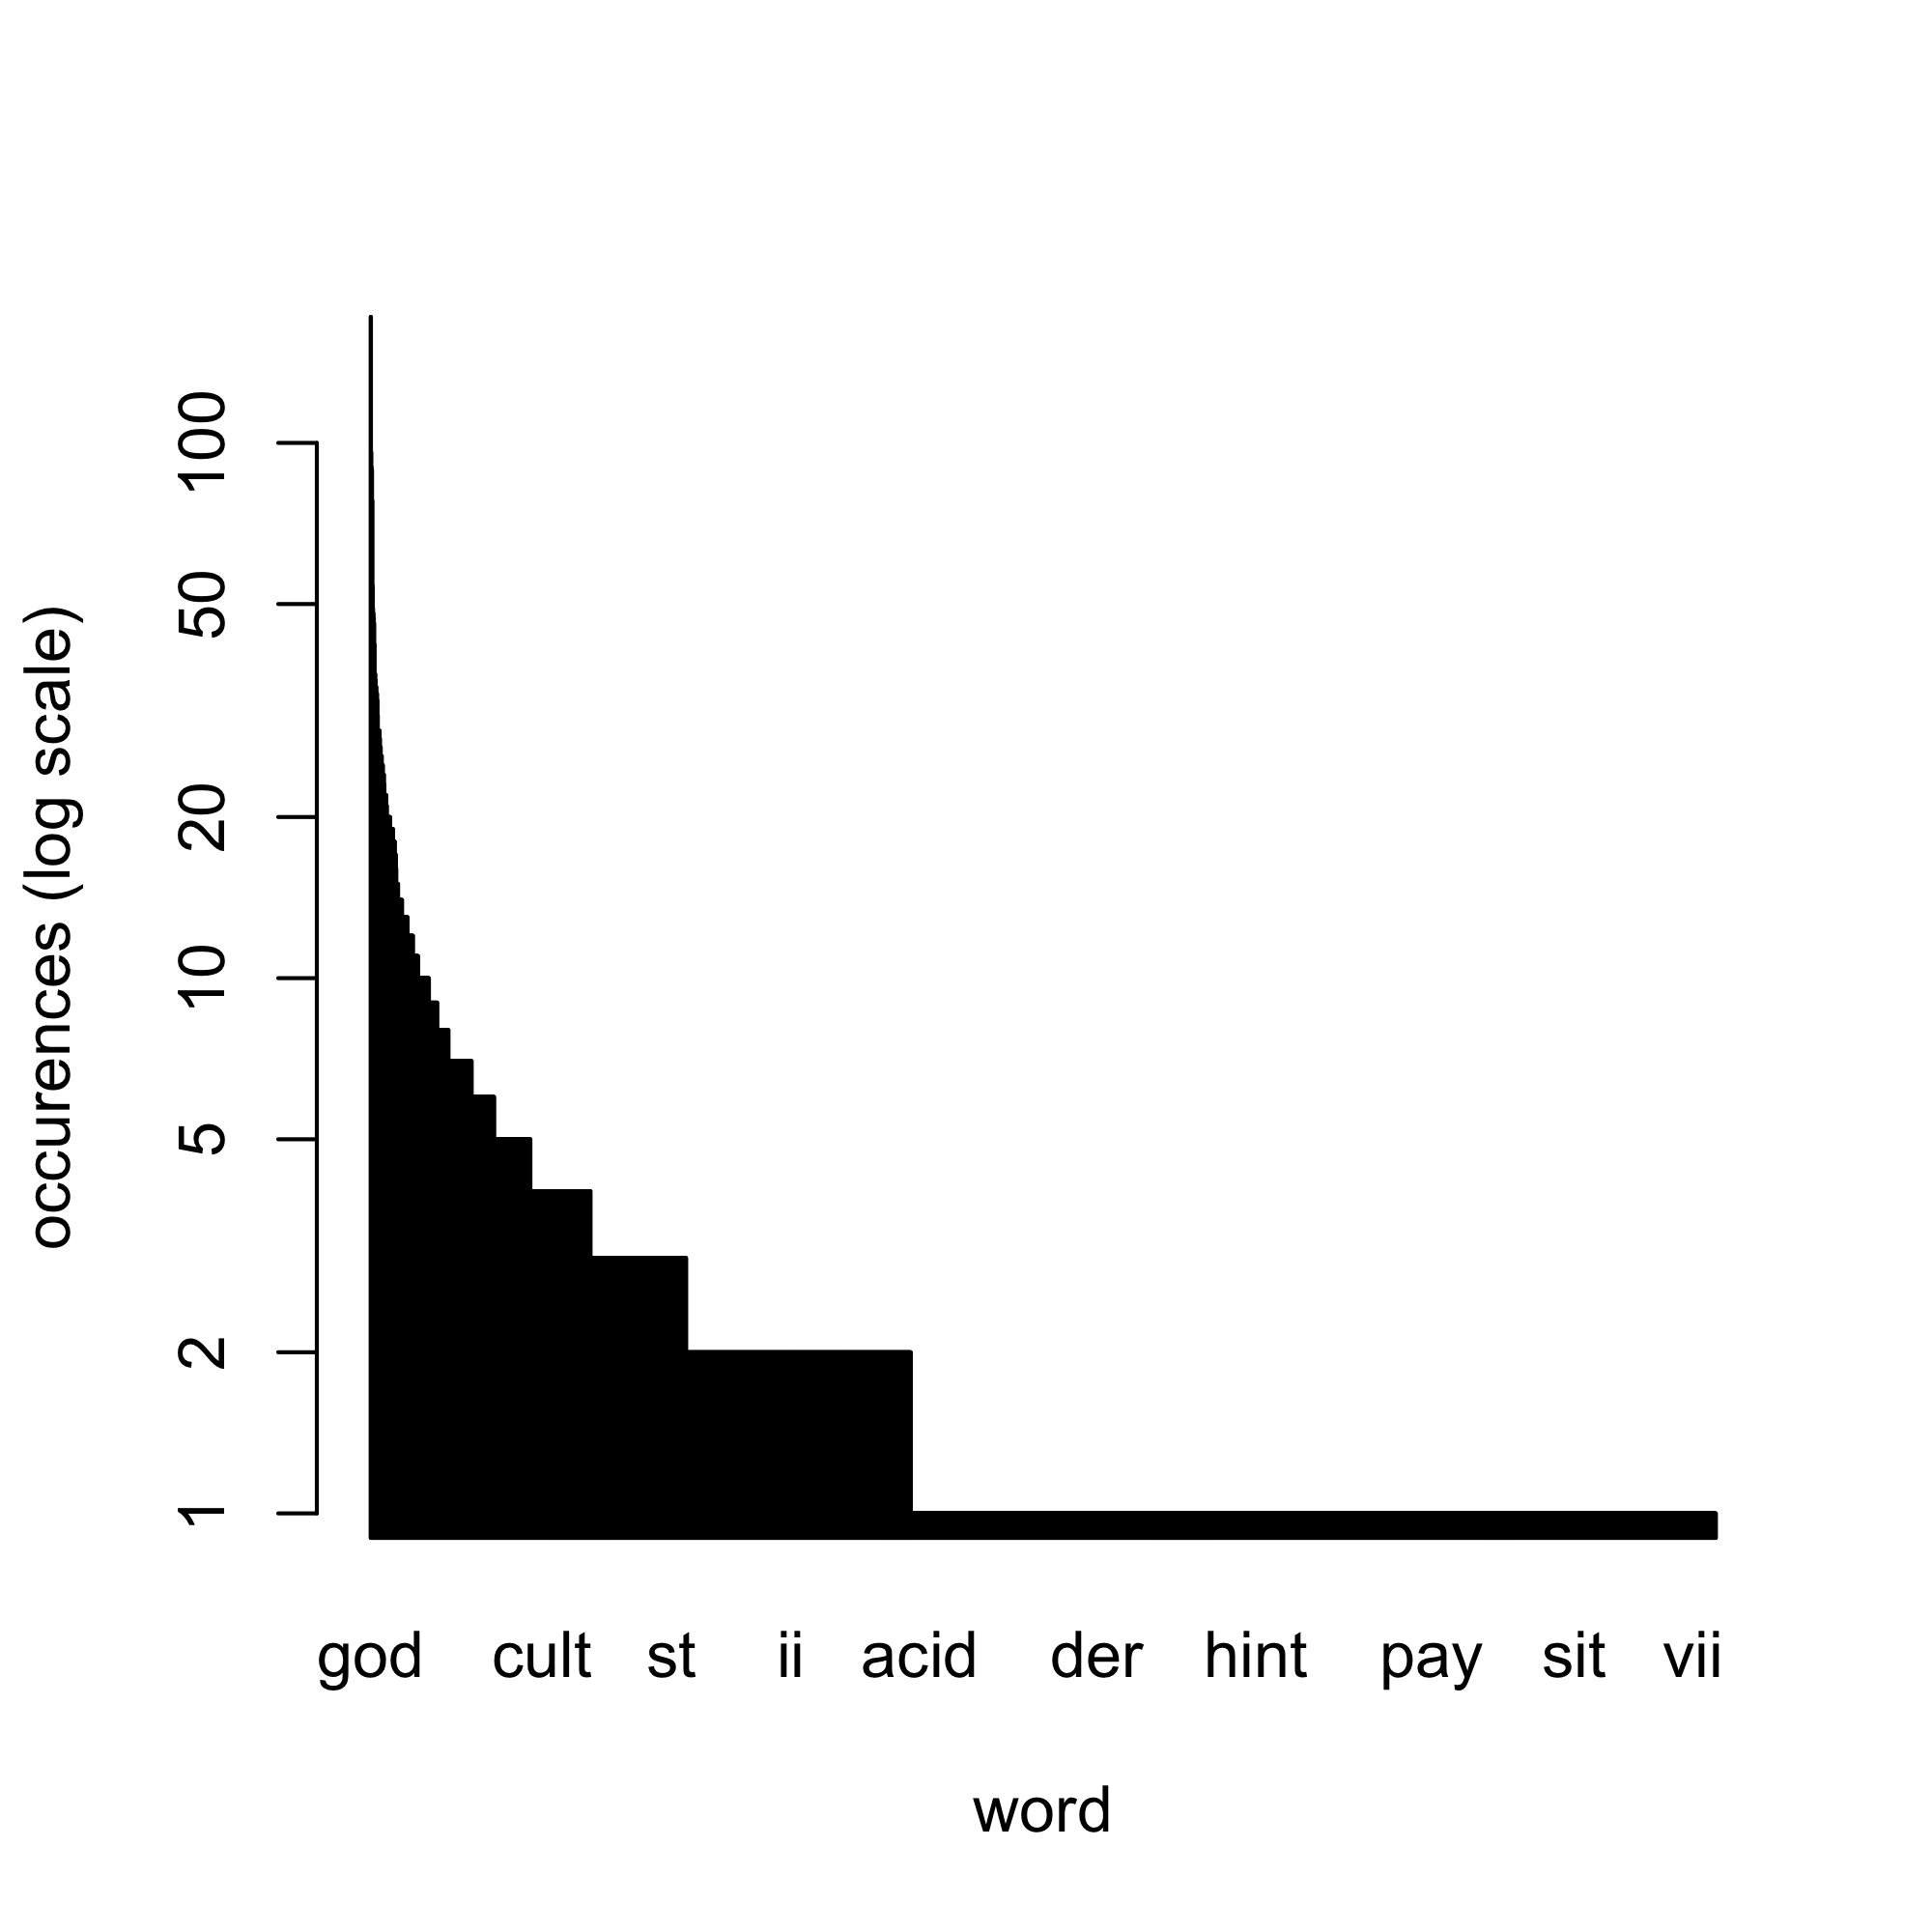
\includegraphics[width=\linewidth]{barplot_words.png}
 	\end{subfigure}
	\begin{subfigure}[b]{0.45\linewidth}
 		\caption{Most-frequent word occurrence.}
 		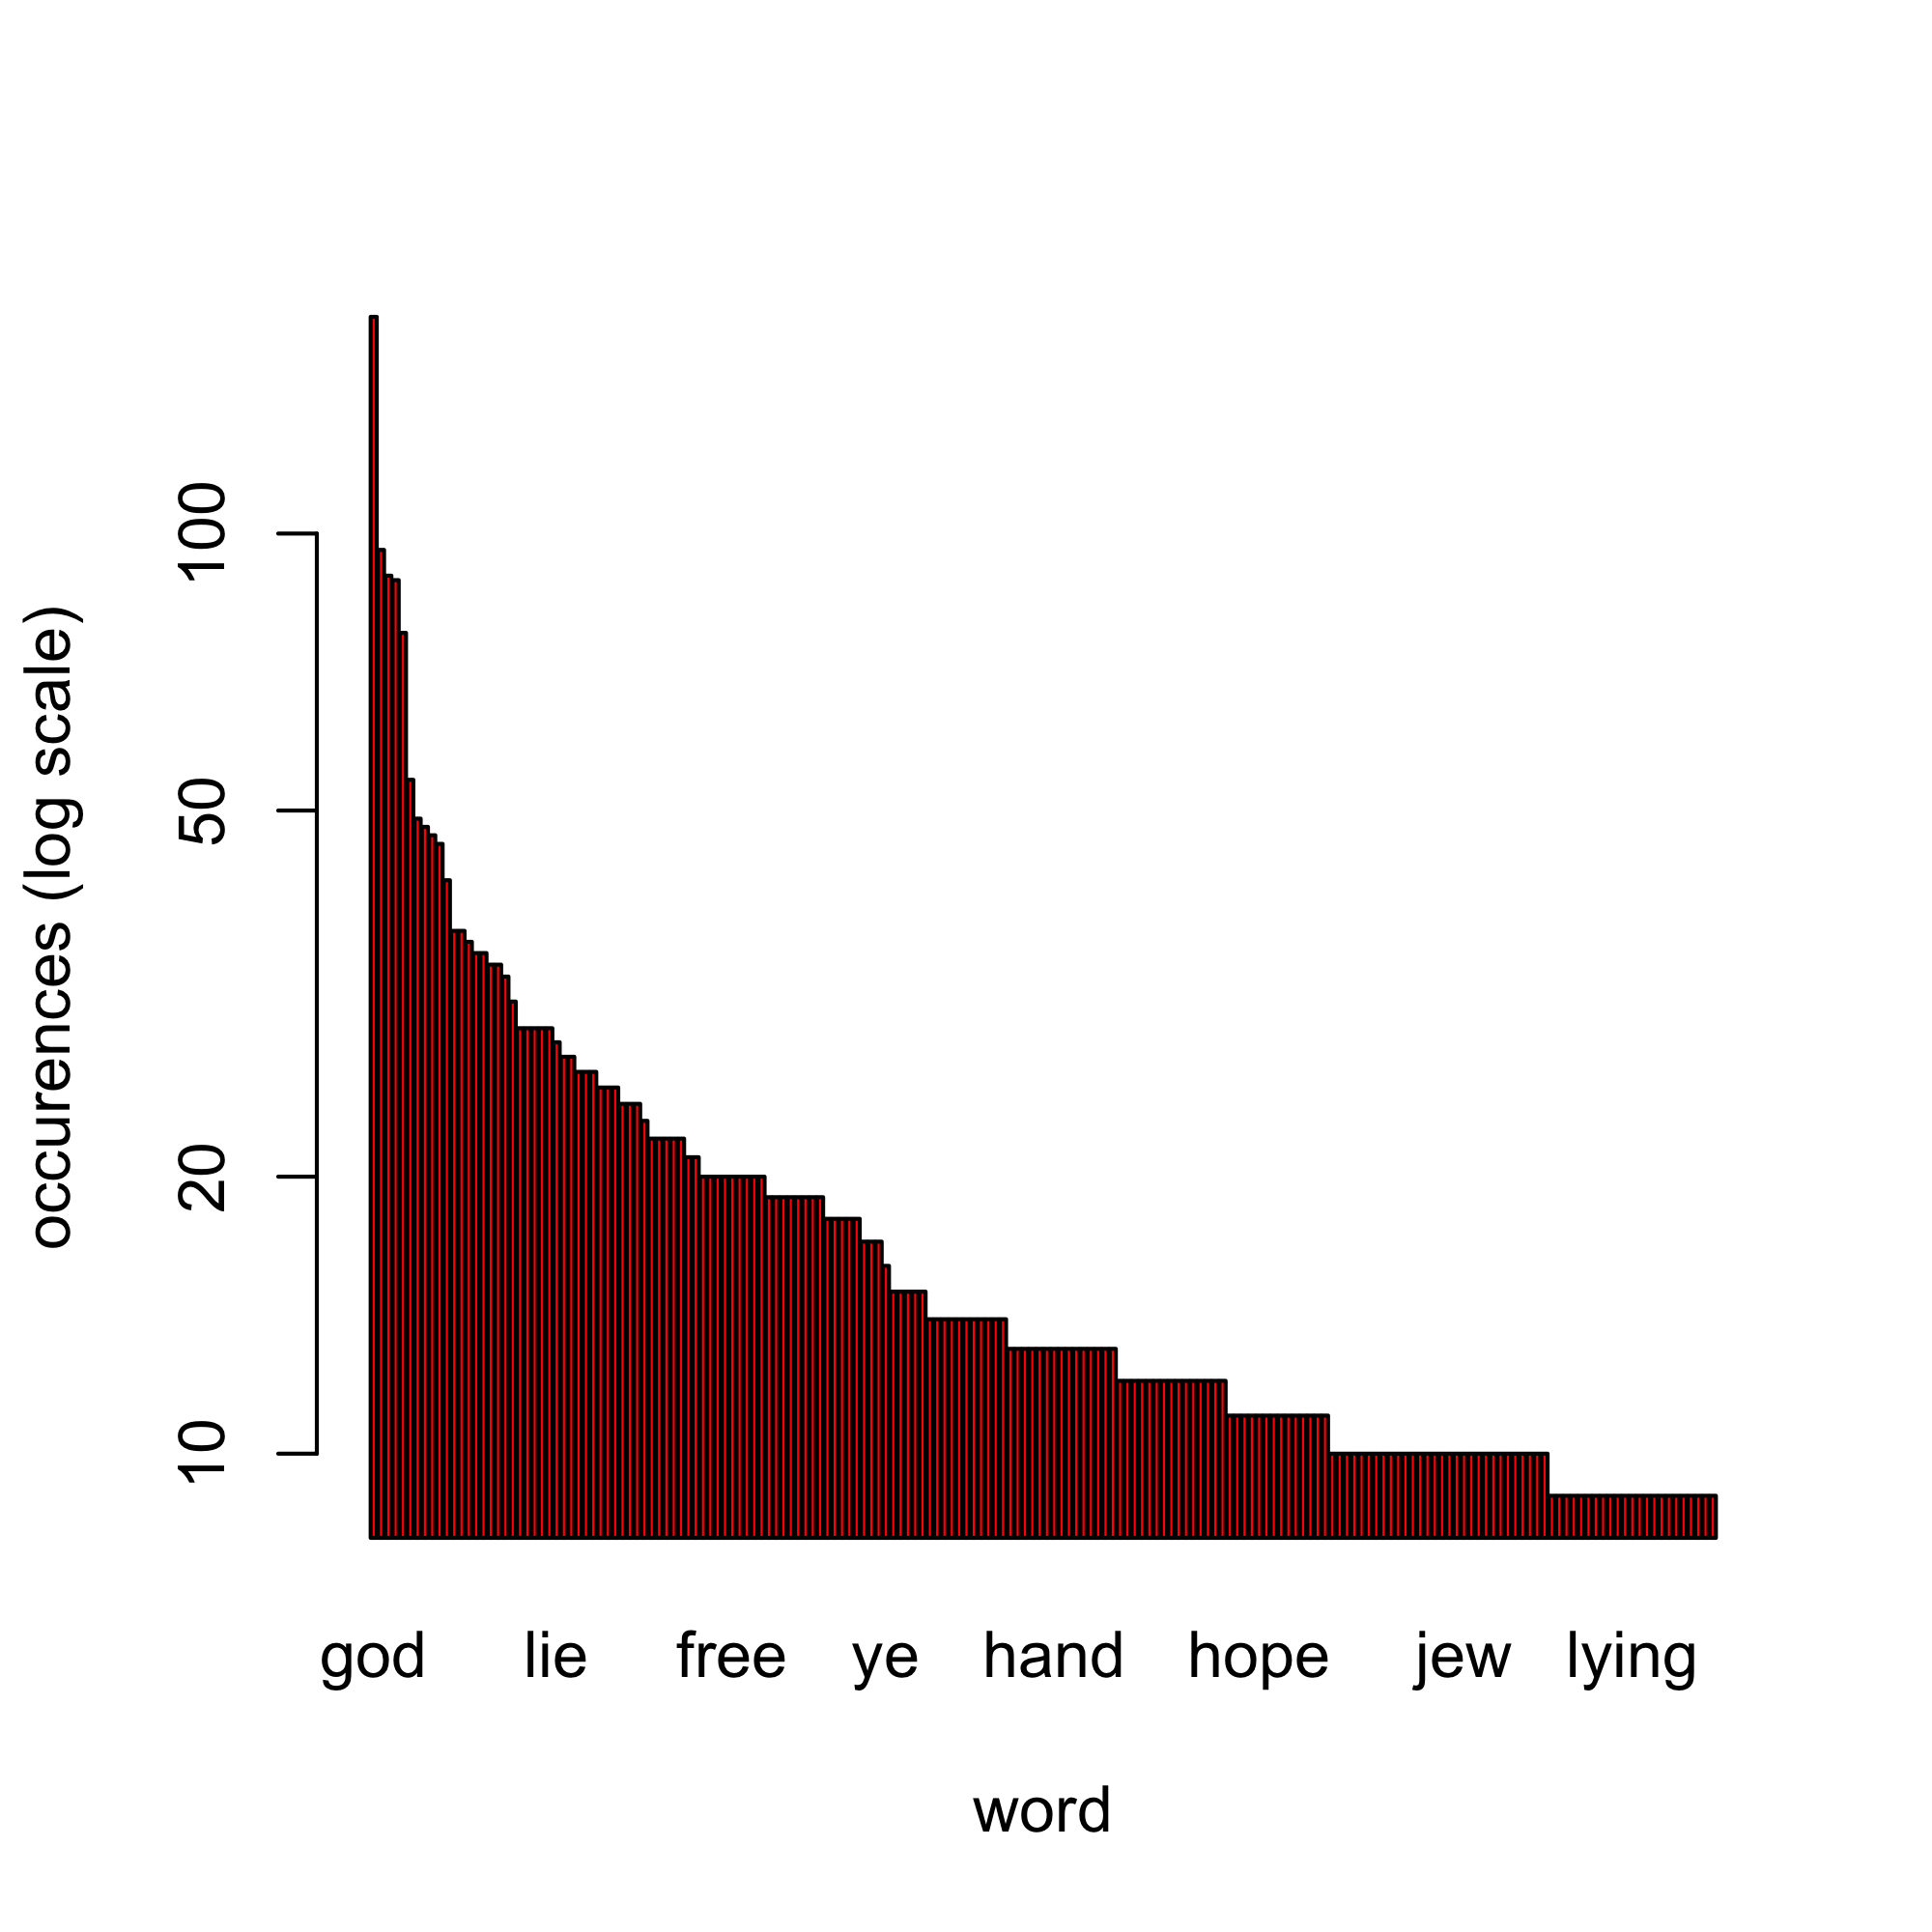
\includegraphics[width=\linewidth]{barplot_freq_words.png}
 	\end{subfigure}
 	\label{fig:barplots_chars_words}
 \end{figure}

\begin{figure}
	\centering
	\caption{Word cloud of the book.}
	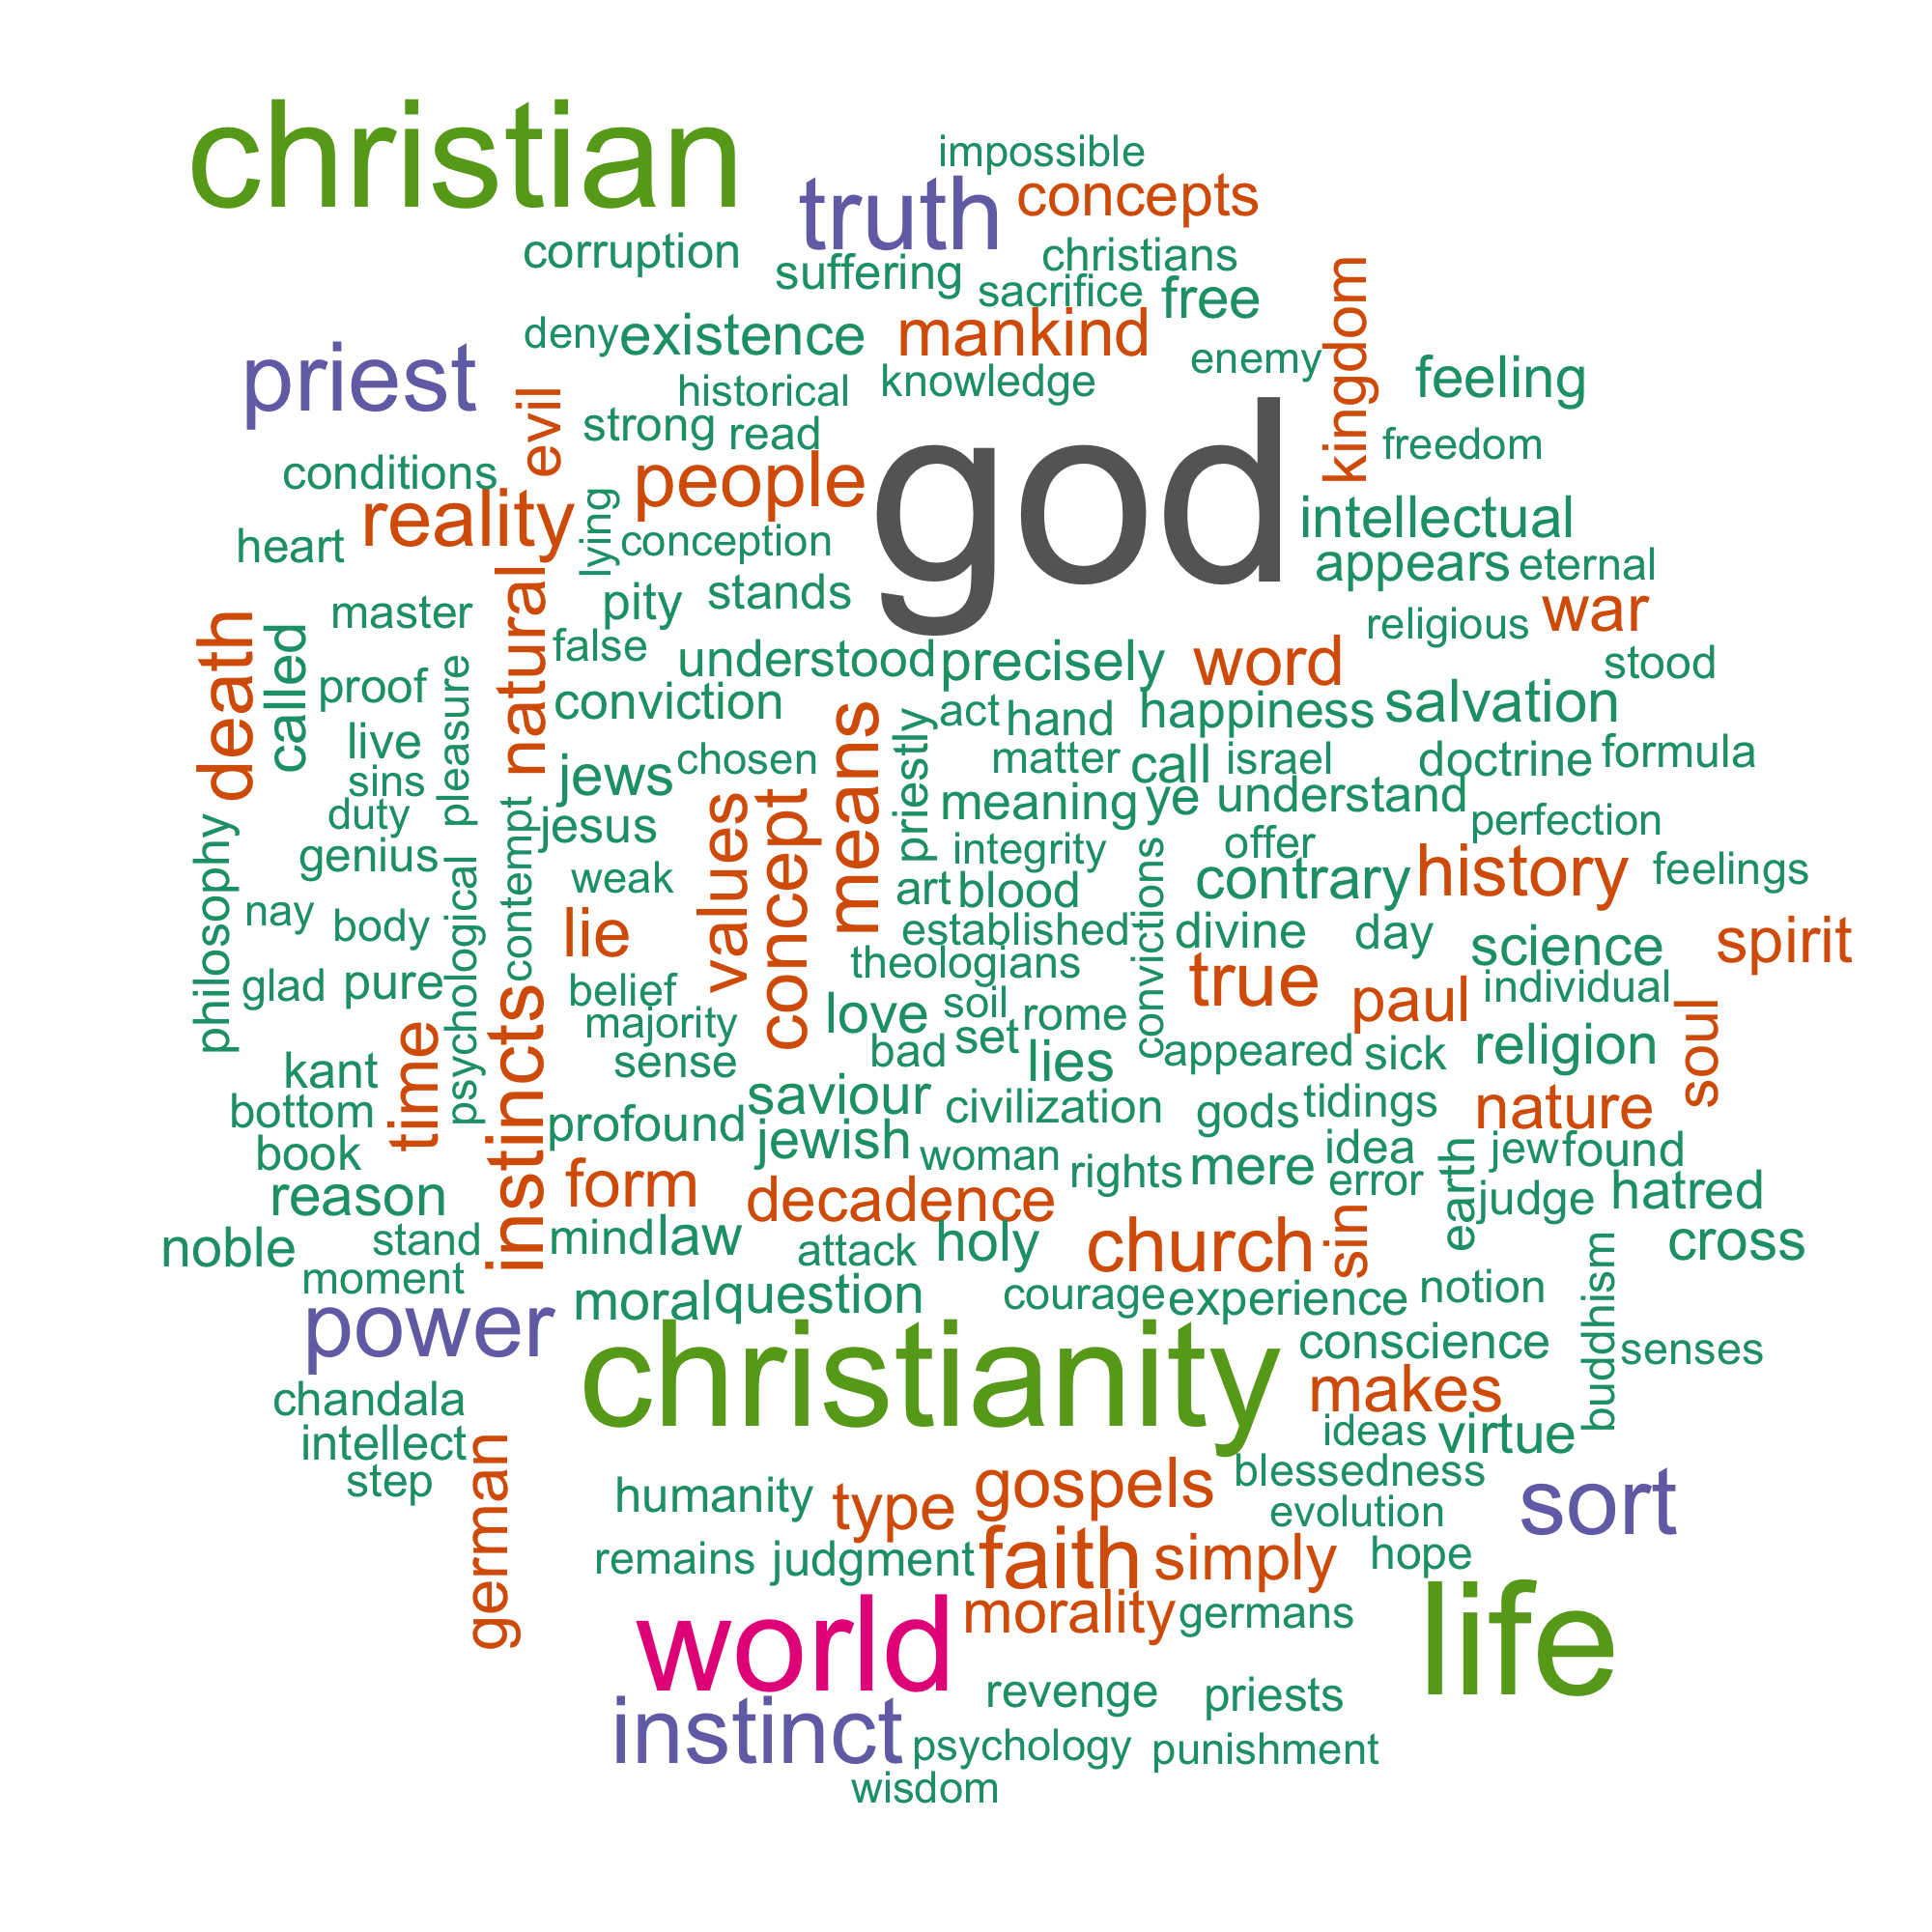
\includegraphics[width=.3 \linewidth]{wordcloud.png}
	\label{fig:wordcloud}
\end{figure}

\subsection{Network representation}
Next, we created a network representation of our text. For readers unfamiliar with network (or graph) theory, basic definitions can be found in Appendix \ref{appendix}. For our analysis, we considered words in the text as our vertices, joining a pair of words with an edge if they appeared together in the text (that is, if they form a bigram). Notice that since every edge joins exactly two words that appeared together in the text, there is a direct correspondence between our edges and the bigrams in the text. We made this a weighted network by assigning to each edge a weight equal to the number of times its corresponding bigram appears in the text. We restricted ourselves to those bigrams appearing more than once. The results can be seen in Figure \ref{fig:network}.  We also extracted the largest connected component of the network, as can be seen in Figure \ref{fig:component}. Vertices with highest degree and strength can be seen in Table \ref{tab:degree-strength}. Finally, we computed the degree distribution of both the whole network and of the largest connected component. The degree distribution gives us the relative frequency of $n$-th degree vertices, with $n = 0, 1, \dots, \max_{v} \lbrace \deg (v) \rbrace$. You can observe these in Figure \ref{fig:degree_distribution}. 

\begin{figure}
	\centering
	\caption{Book network representation.} 
	\begin{subfigure}{0.45\linewidth}
		\caption{Network with words as vertices and edges joining words appearing as a bigram in the text.}
		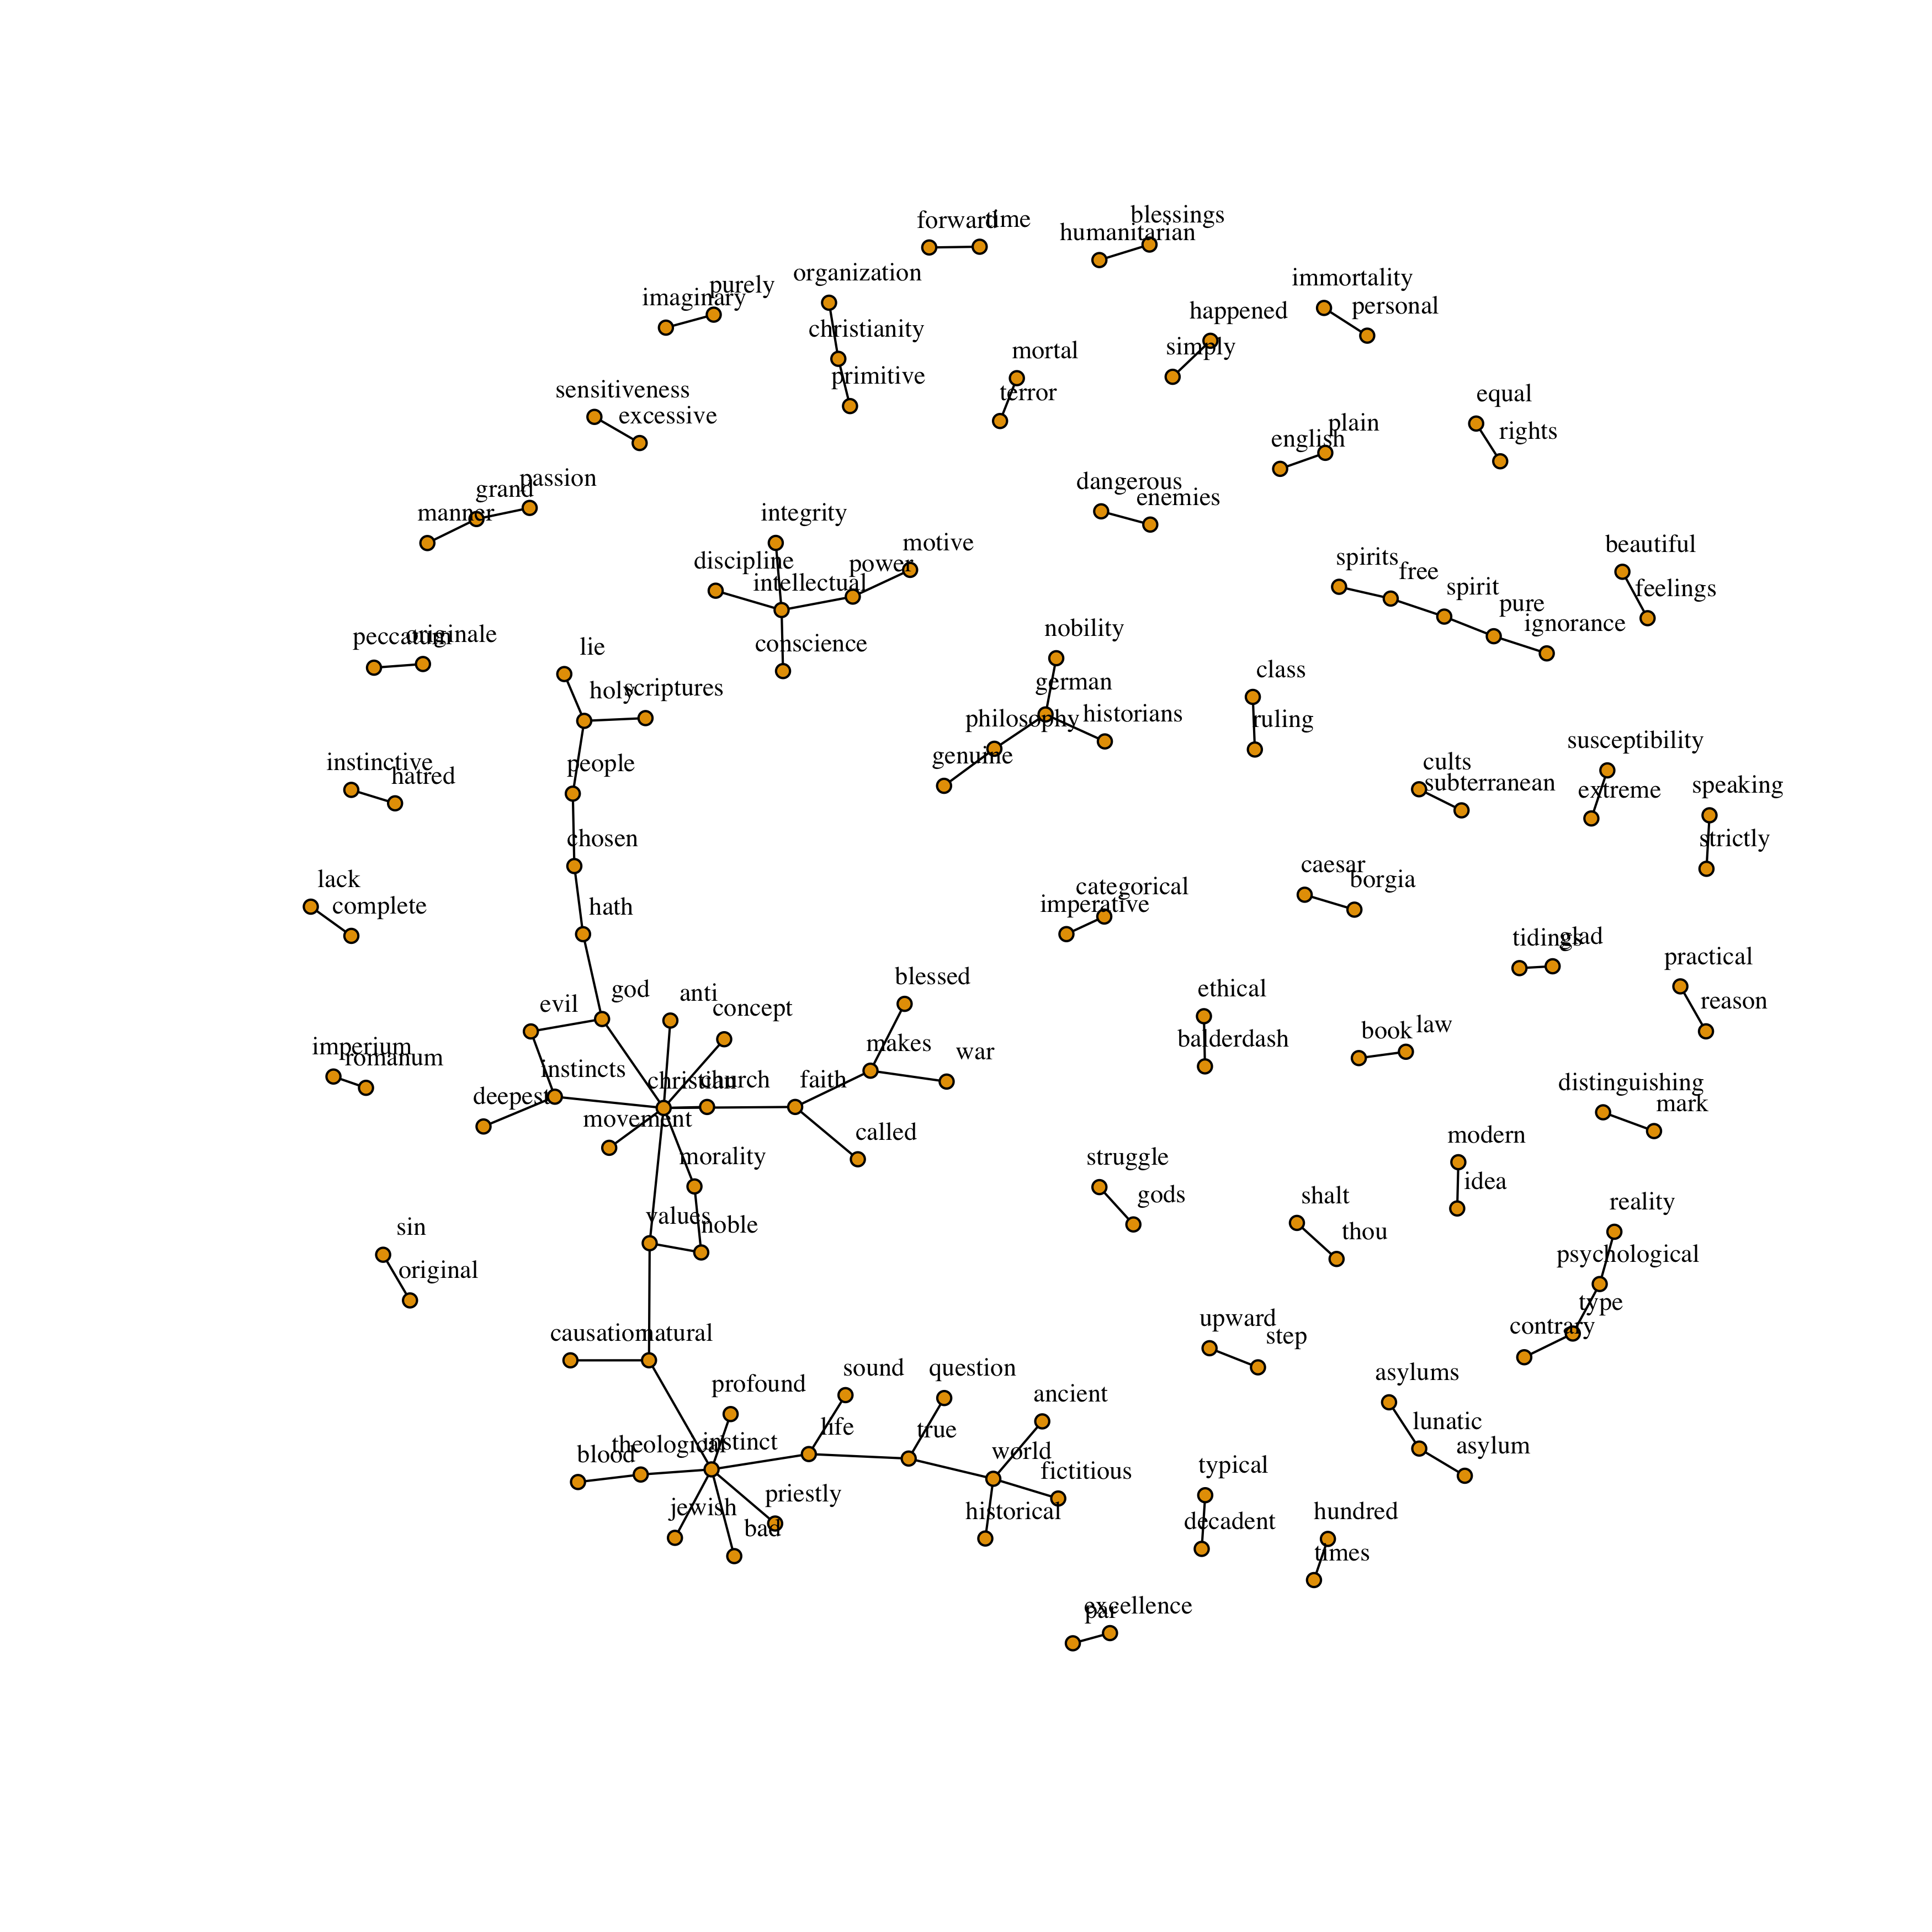
\includegraphics[width=\linewidth]{bigram_network.png}
	\end{subfigure}
	\hfill
	\begin{subfigure}{0.45\linewidth}
		\caption{Same network, with vertex size and edge width proportional to their degree and weight.}
		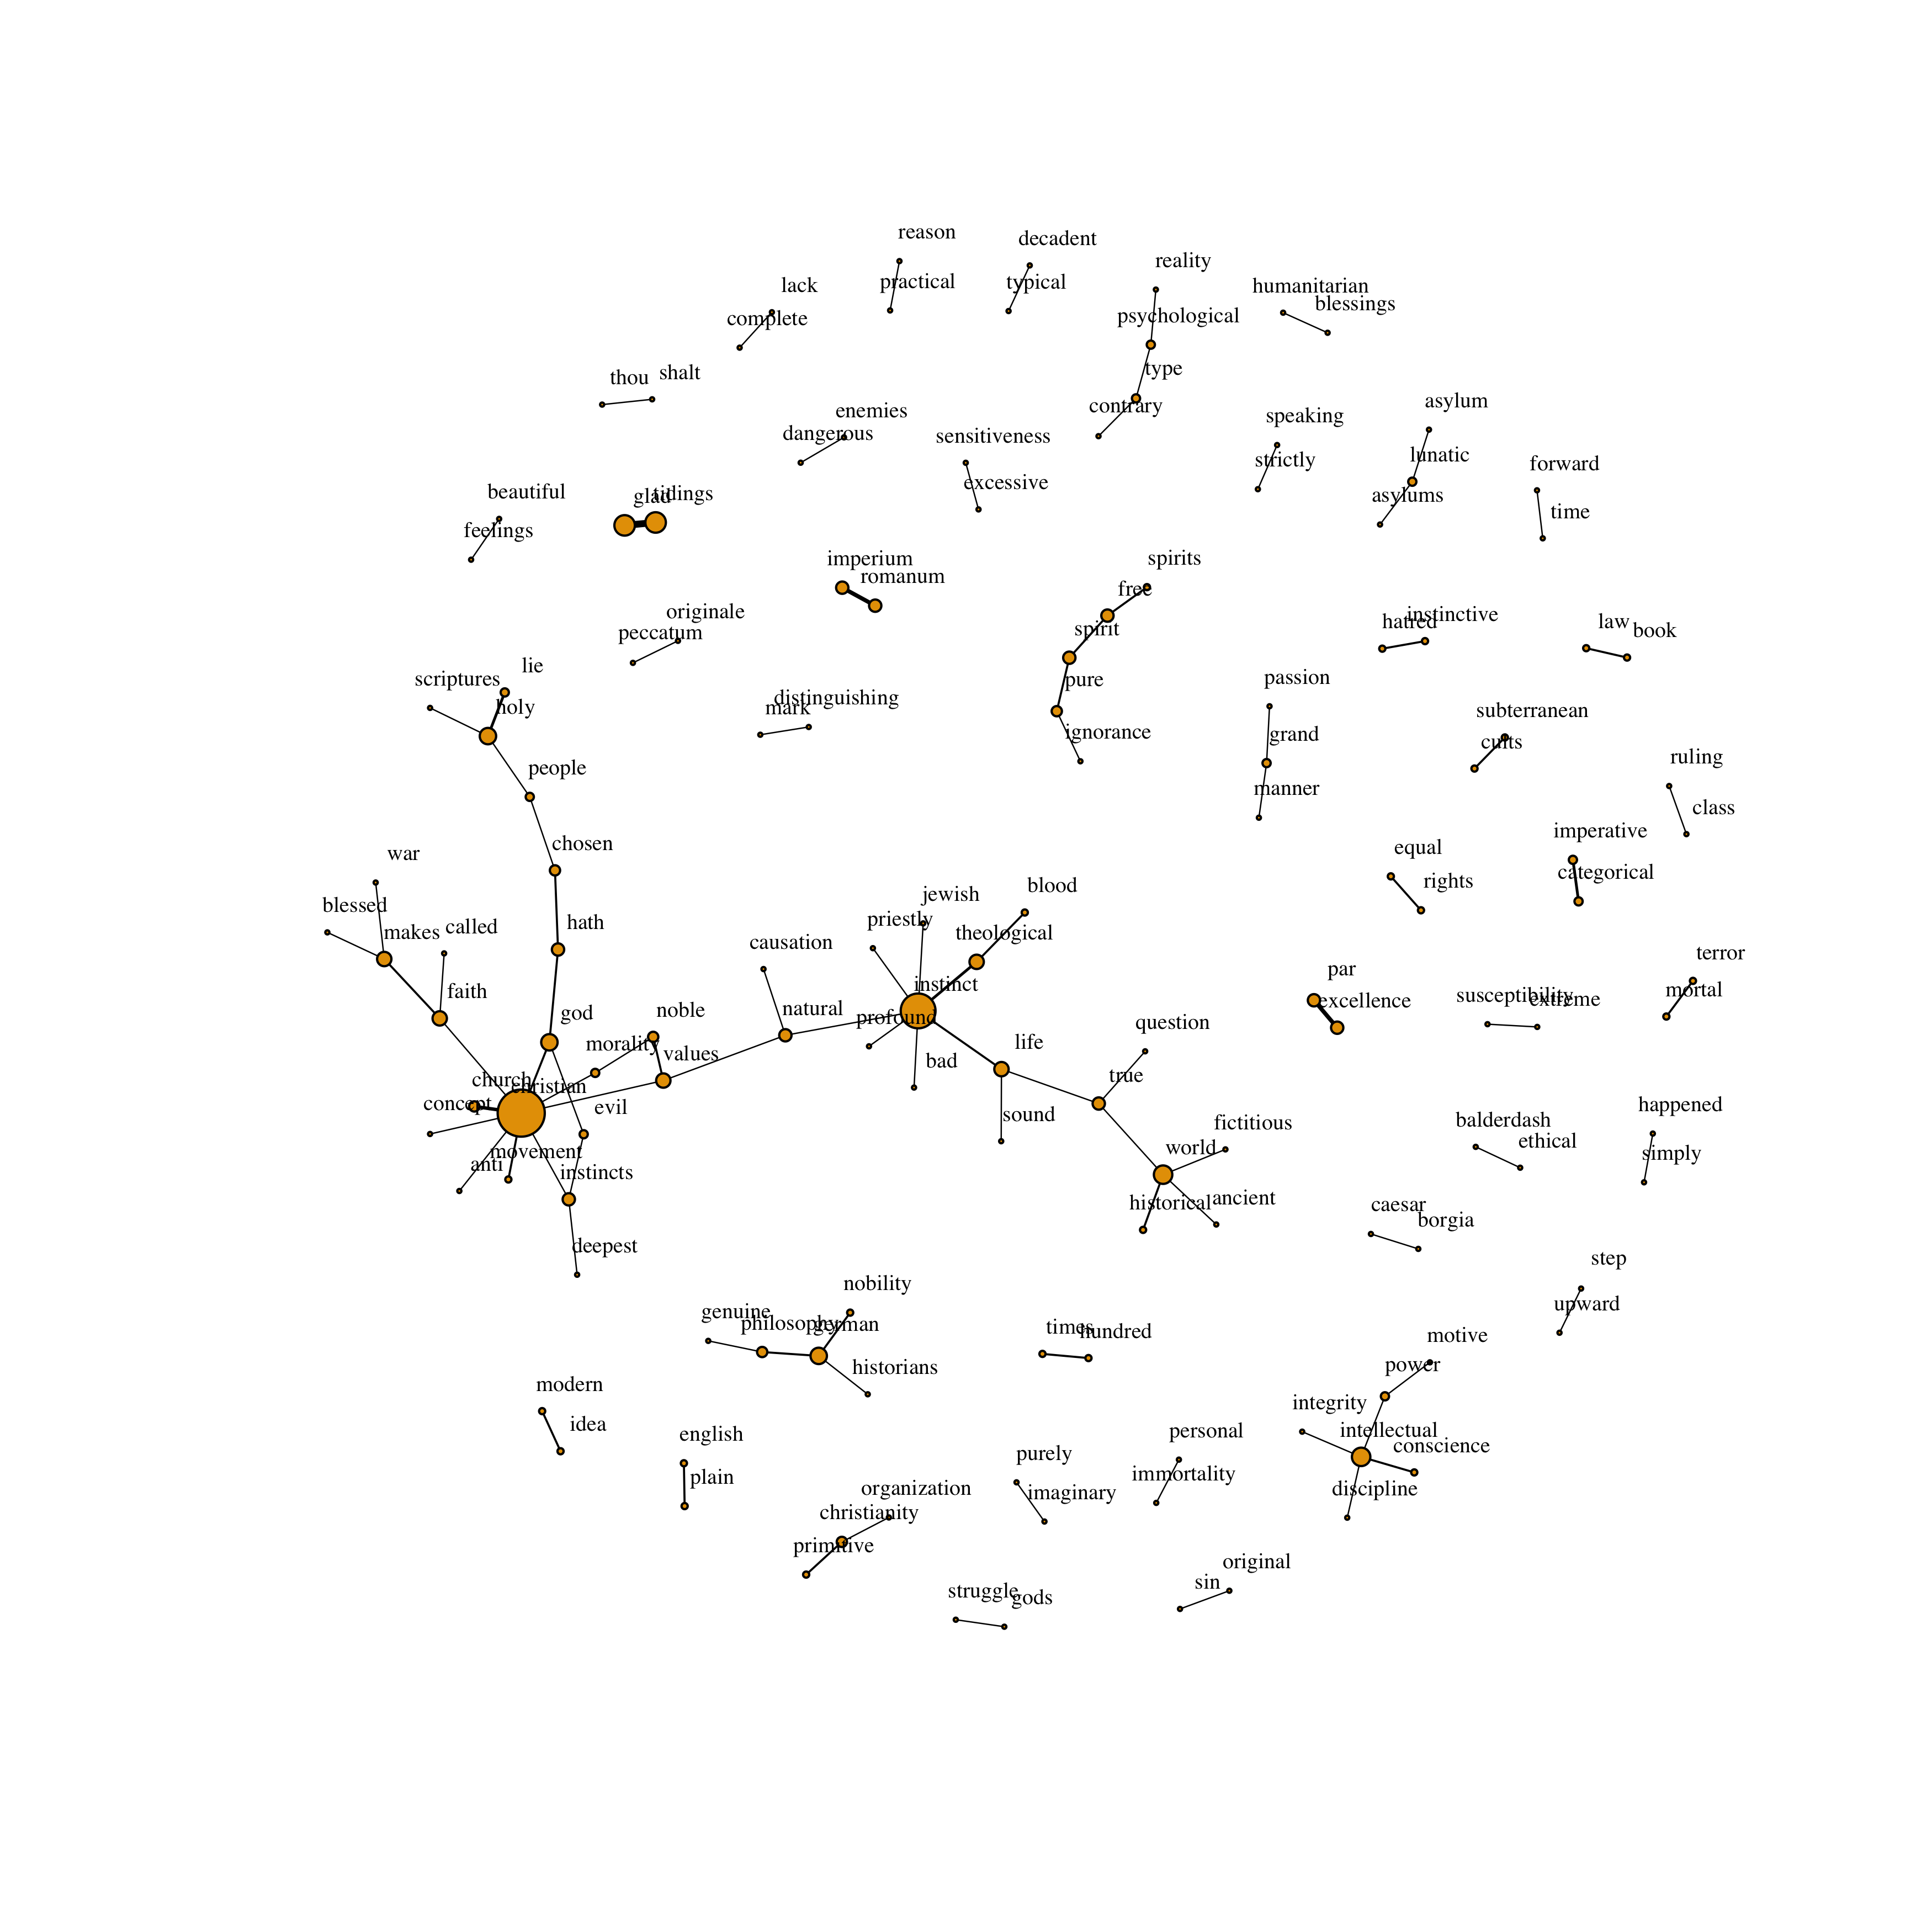
\includegraphics[width=\linewidth]{bigram_network_2.png}
	\end{subfigure}
	\label{fig:network}
\end{figure}


\begin{figure}
	\centering
	\caption{Largest component of network in Figure \ref{fig:network}, with vertex sizes and edges width proportional to their degree and weight.}
		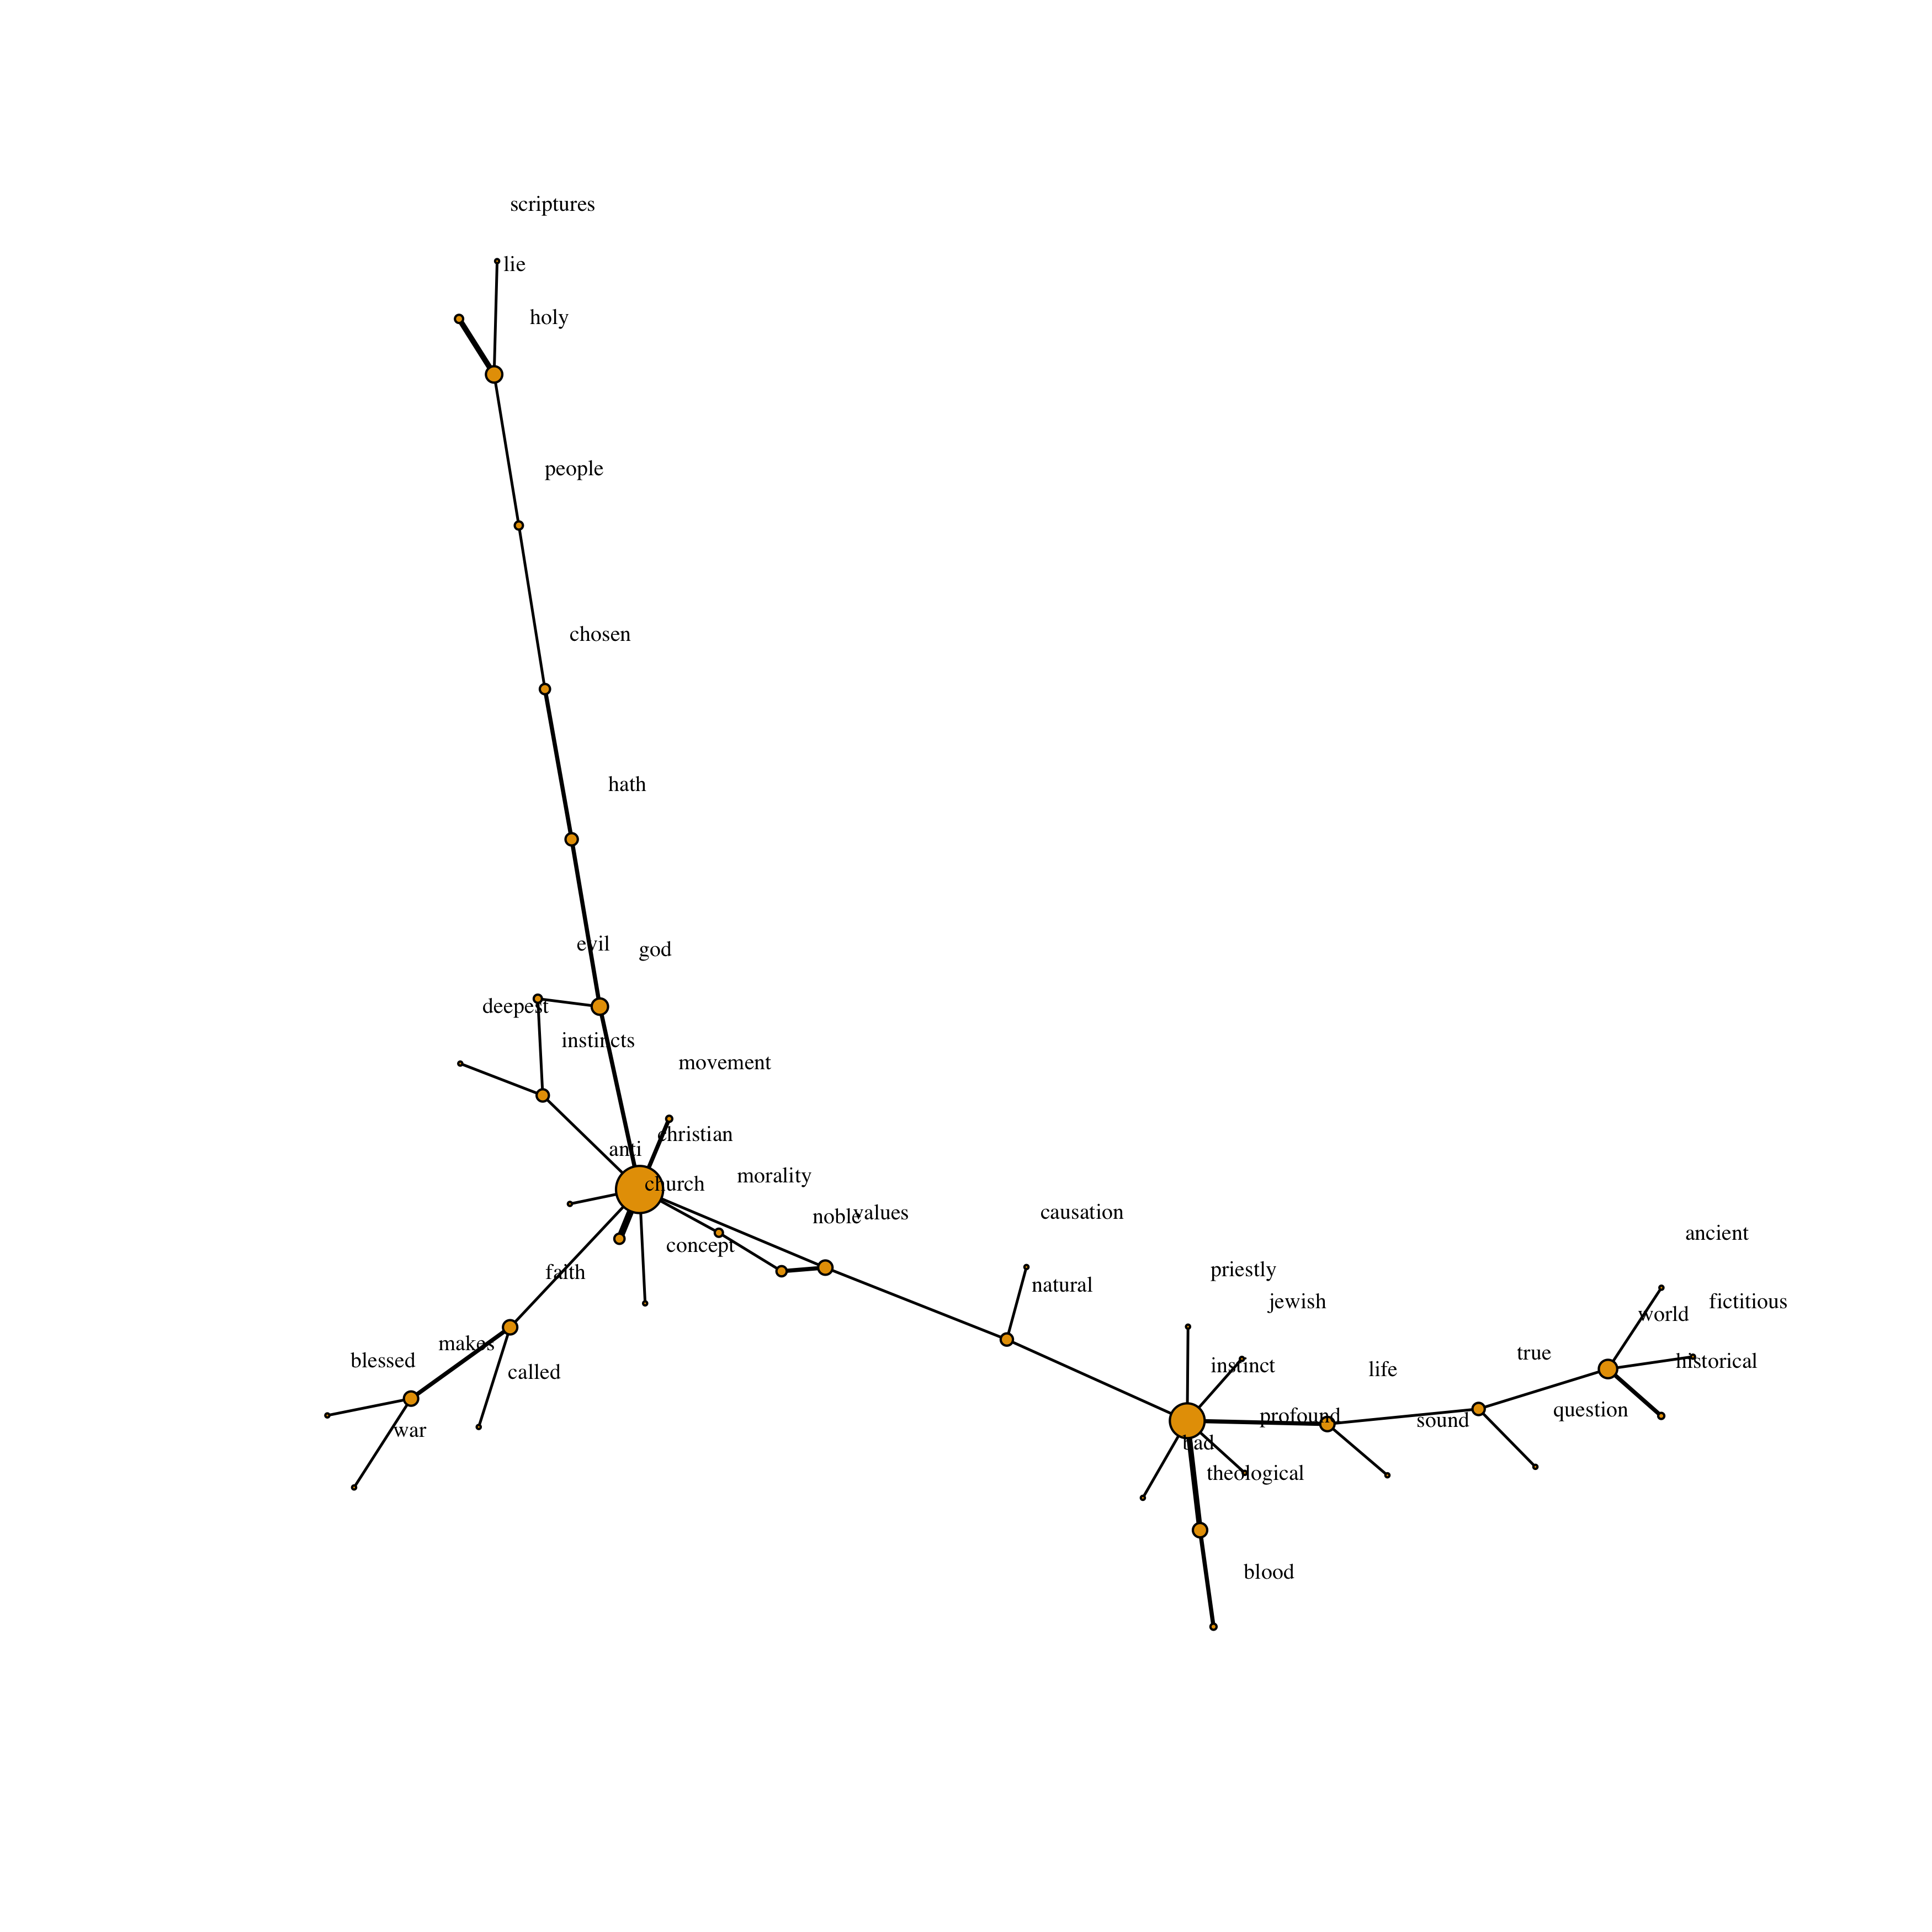
\includegraphics[width=.6 \linewidth]{bigram_component.png}
	\label{fig:component}
\end{figure}

\begin{figure}
	\centering
	\caption{Degree distributions.} 
	\begin{subfigure}{0.45\linewidth}
		\caption{Relative frequency of $n$th degree vertices in our network.}
		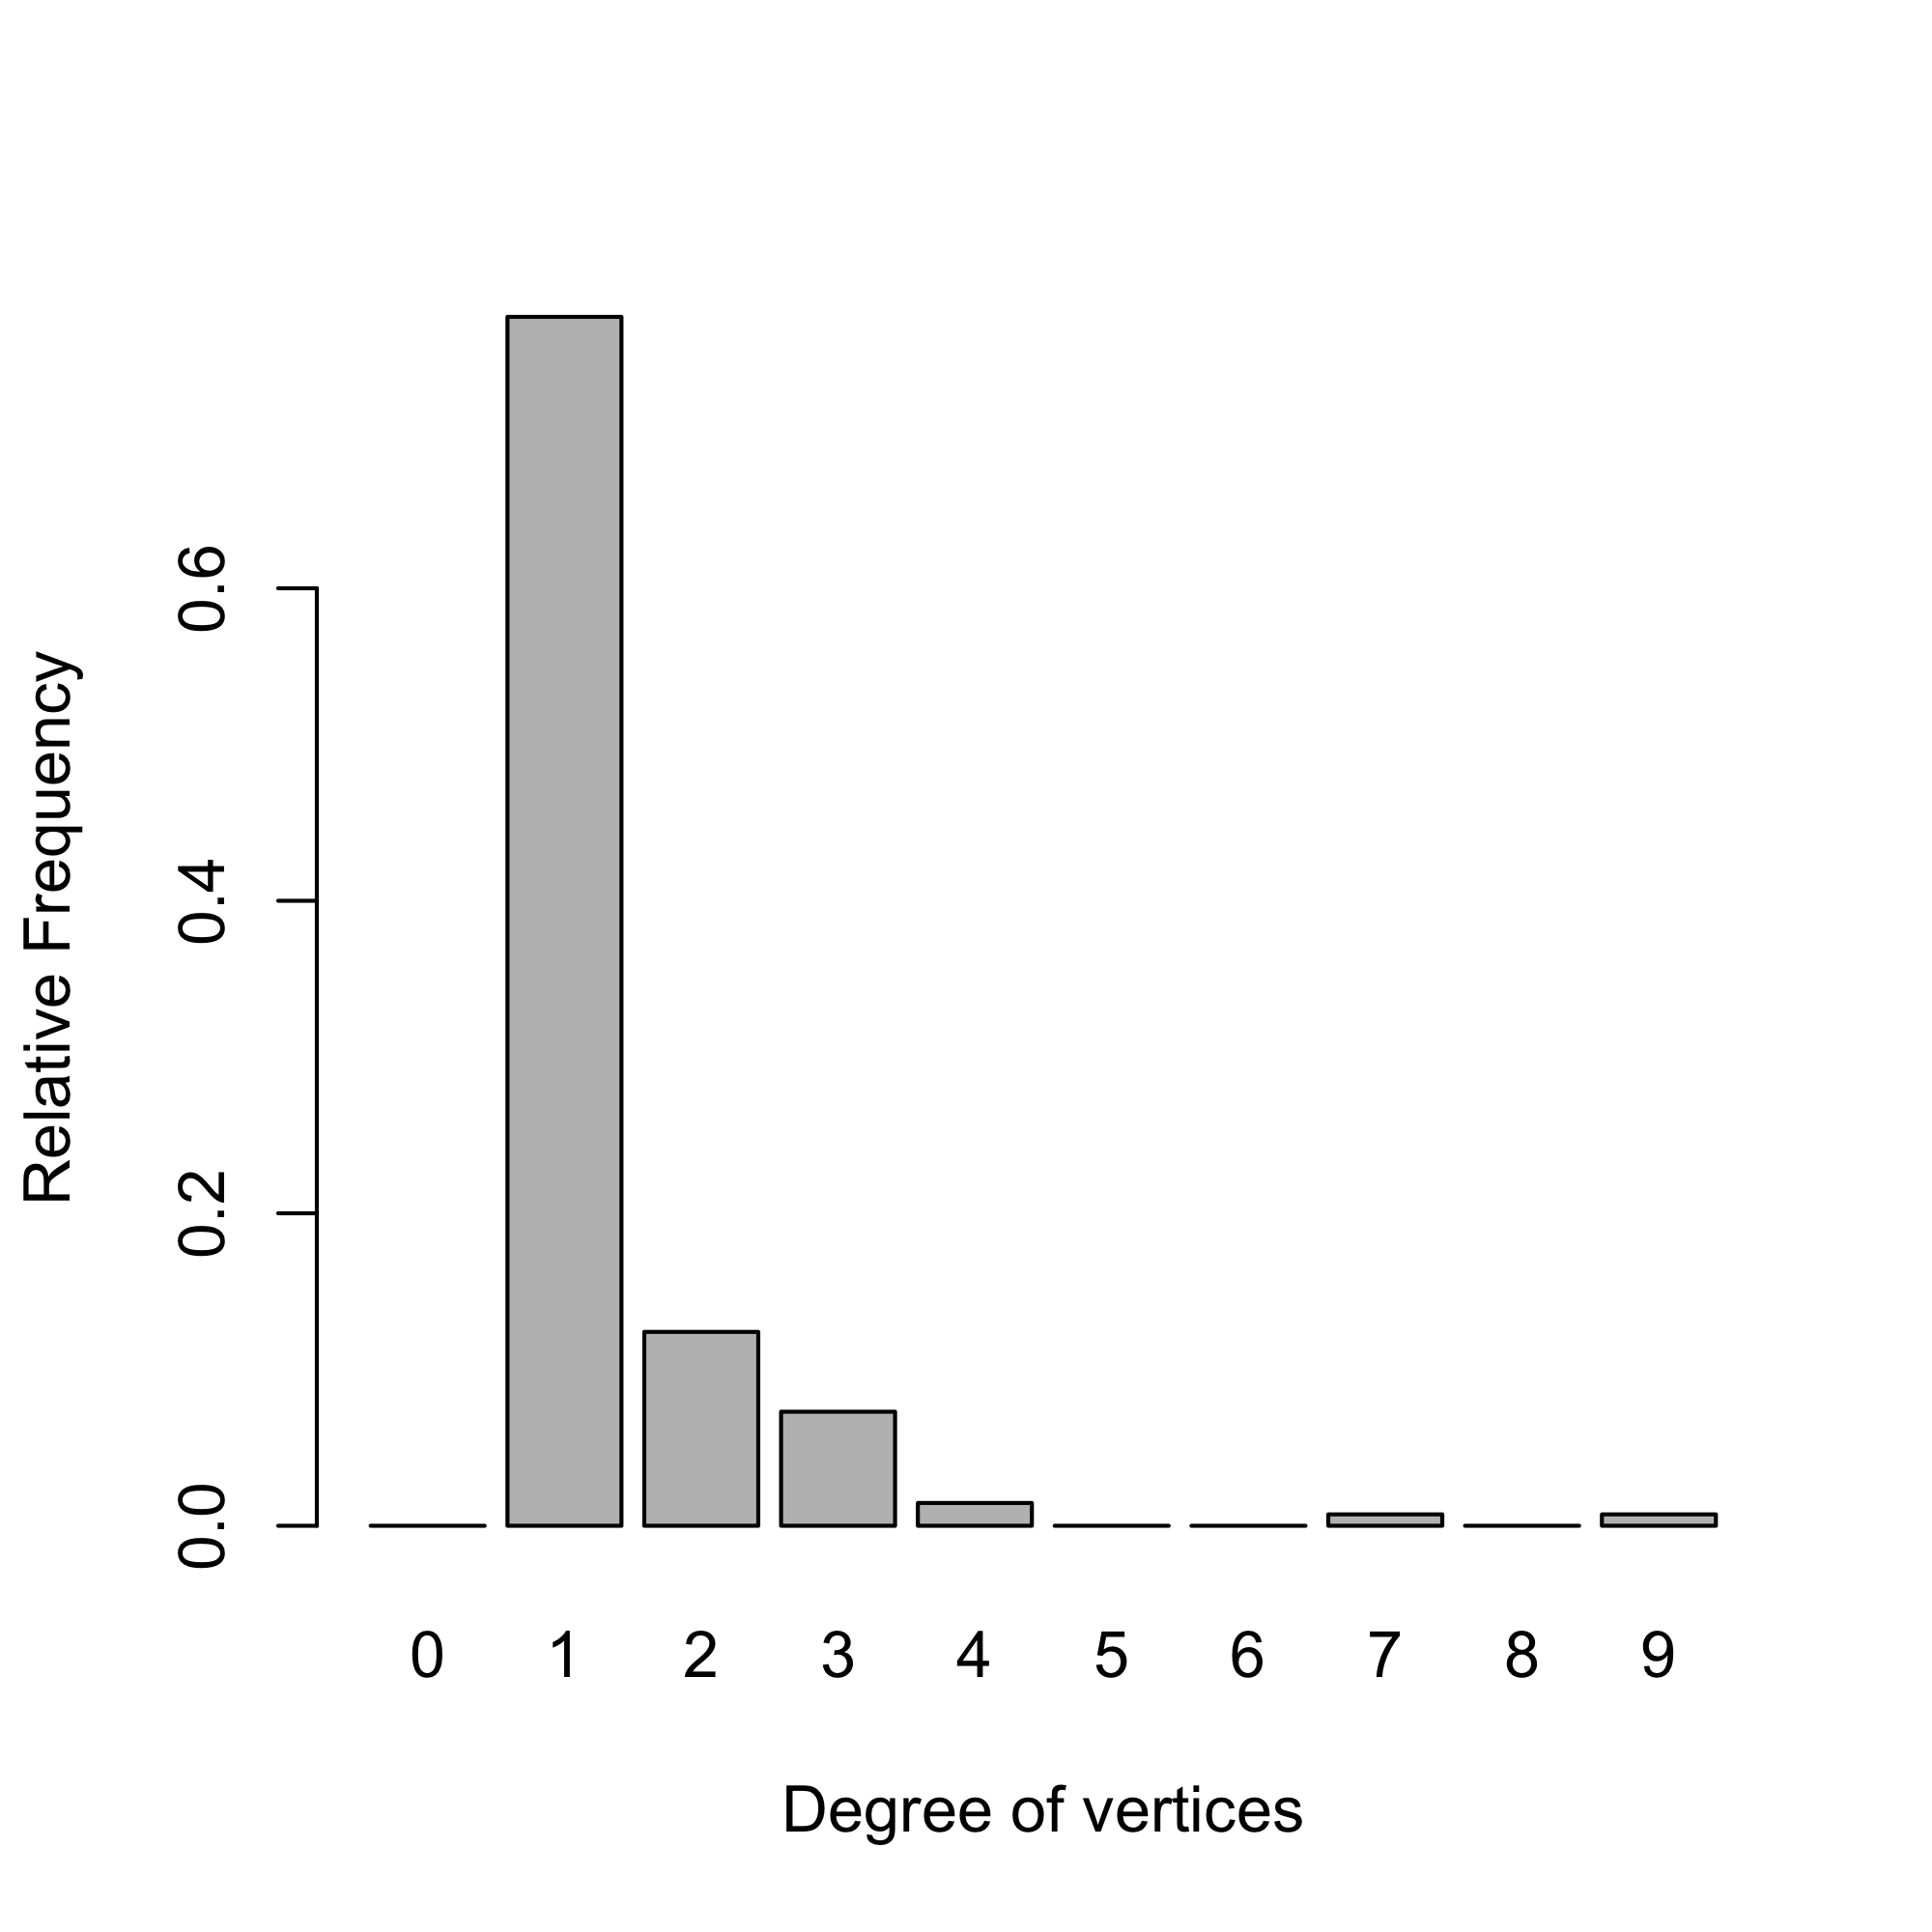
\includegraphics[width=\linewidth]{network_degree_distribution.png}
	\end{subfigure}
	\hfill
	\begin{subfigure}{0.45\linewidth}
		\caption{Relative frequency of $n$th degree vertices in the network's largest component.}
		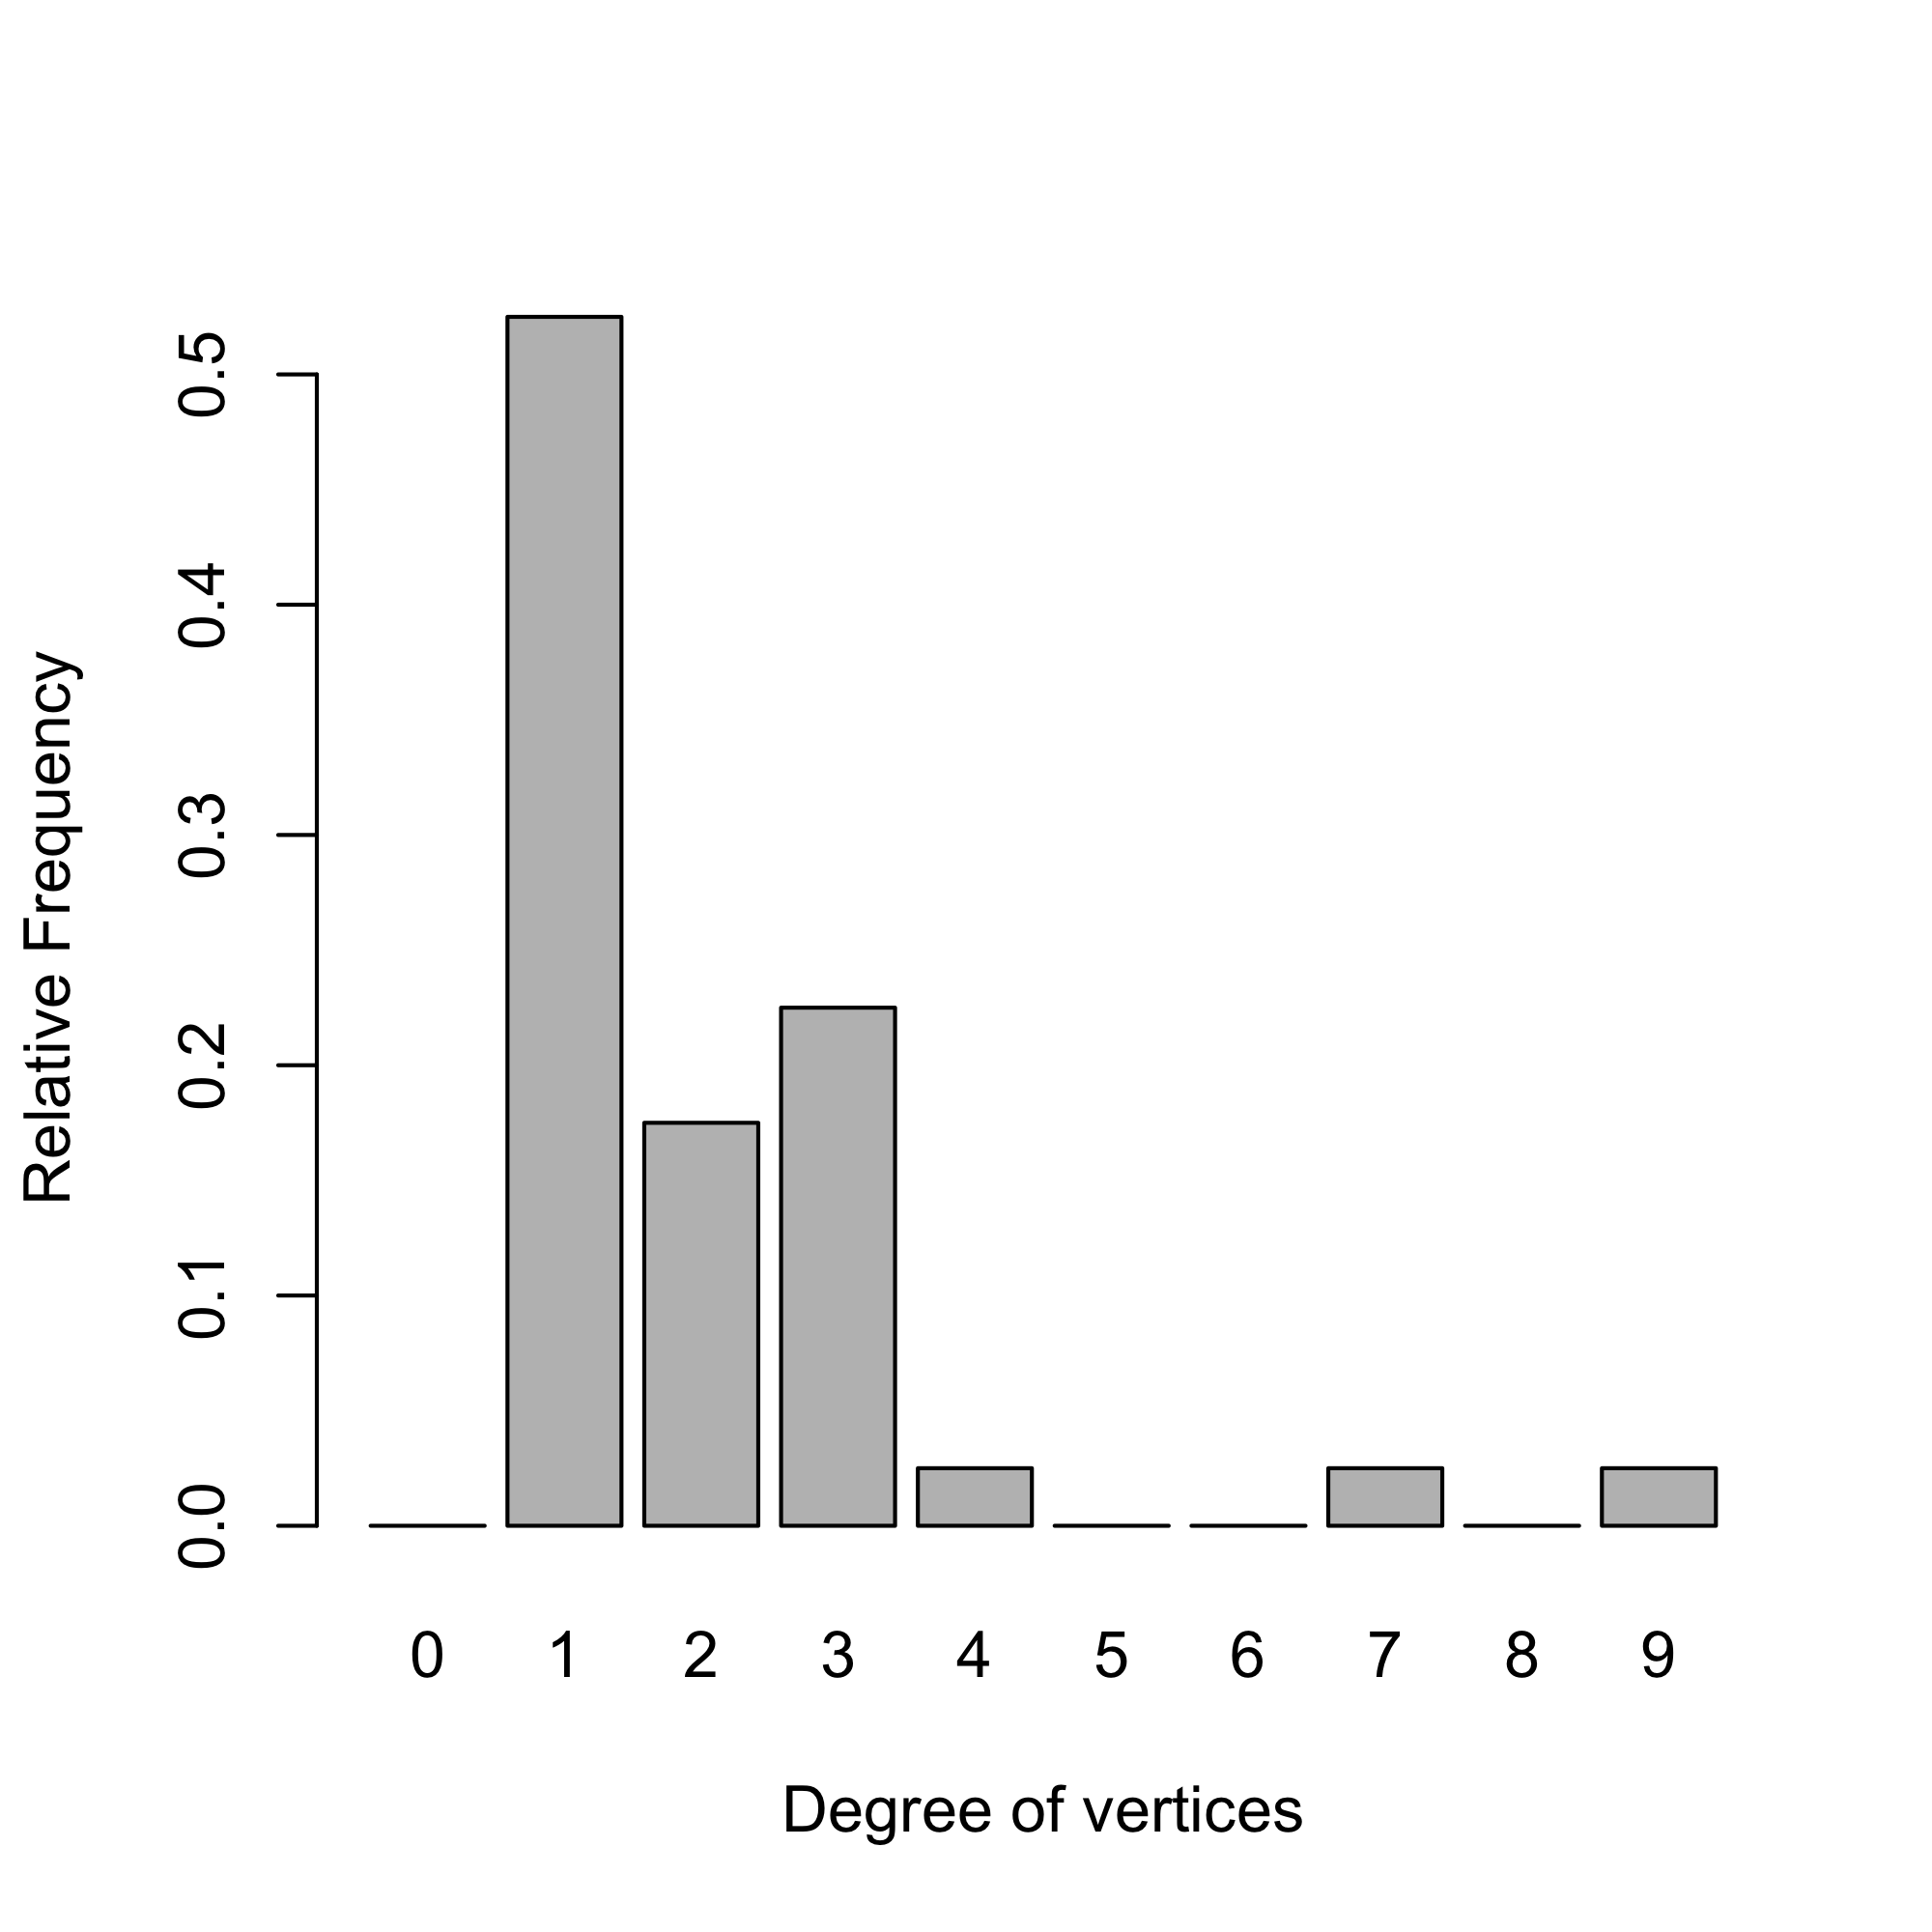
\includegraphics[width=\linewidth]{component_degree_distribution.png}
	\end{subfigure}
	\label{fig:degree_distribution}
\end{figure}

\begin{table}
	\caption{Highest degree and strength vertices for largest connected component in the network.}
	\begin{subtable}[ht]{0.45\textwidth}
		\centering
		\caption{Sorted by degree.}
		\centering
		\begin{tabular}{lrr}
			\hline
			vertex & degree & strength \\ 
			\hline
			christian & 9.00 & 23.00 \\ 
			instinct & 7.00 & 17.00 \\ 
			world & 4.00 & 9.00 \\ 
			holy & 3.00 & 8.00 \\ 
			faith & 3.00 & 7.00 \\ 
			god & 3.00 & 8.00 \\ 
			life & 3.00 & 7.00 \\ 
			makes & 3.00 & 7.00 \\ 
			natural & 3.00 & 6.00 \\ 
			true & 3.00 & 6.00 \\ 
			\hline
		\end{tabular}
	\end{subtable}
	\hfill
	\begin{subtable}[ht]{0.45\textwidth}
		\centering
		\caption{Sorted by strength}
			\centering
			\begin{tabular}{lrr}
				\hline
				vertex & degree & strength \\ 
				\hline
				christian & 9.00 & 23.00 \\ 
				instinct & 7.00 & 17.00 \\ 
				world & 4.00 & 9.00 \\ 
				holy & 3.00 & 8.00 \\ 
				god & 3.00 & 8.00 \\ 
				theological & 2.00 & 7.00 \\ 
				faith & 3.00 & 7.00 \\ 
				life & 3.00 & 7.00 \\ 
				makes & 3.00 & 7.00 \\ 
				values & 3.00 & 7.00 \\ 
				\hline
			\end{tabular}
	\end{subtable}
	\label{tab:degree-strength}
\end{table}

\section{Conclusion}
In accordance to what was expected given the theme of the book, the words \textit{god}, \textit{life}, \textit{christian} and \textit{christianity} appear the most in the text. The word \textit{christian} is also the highest-degree word in our network. It is of interest to observe that while \textit{instinct} is the 9th most appearing word, is the second word with highest degree (and strength) in our network. This means that, while overall is not the most used, it is still very \textquotedblleft central\textquotedblright in joining words together. These are all very elementary findings. More sophisticated techniques can still be used to get a deeper study of Nietzsche's work, e.g., sentiment analysis. Further work can involve the comparison of different Nietzsche's books, or comparison of Nietzsche's books with works of other authors, in an attempt to characterize his writing style.

\appendix
\section{Network theory} \label{appendix}
 The following theory, and more about networks, can be found at Jungnickel's book\cite{jungnickel}. A \textit{network} (or \textit{graph} in the mathematics literature) is a pair $\N = (V, E)$ consisting of a non-empty, finite set $V$ and a set $E$ of two-element subsets of $V$\footnote{Some literature allows $V$ to be infinite, but it will not be needed in our discussion. Also, for \textit{directed} networks, $E$ consists of ordered pairs of elements of $V$.}. An element $e = \lbrace a, b\rbrace \in E$ is called an \textit{edge} with \textit{end vertices} $a$ and $b$. We say that $a$ and $b$ are \textit{incident} with $e$ and that $a$ and $b$ are \textit{adjacent} or \textit{neighbors} of each other, and write $e = ab$. The degree of a vertex $v$ is defined as 
\begin{equation}
\deg v := | \lbrace u \in V : u \text{ is adjacent to v } \rbrace |,
\end{equation} 
where $|A|$ denotes the cardinality of a set $A$. A network is \textit{weighted} if there is a function $w: E \rightarrow \mathbb{R}$, and we say and edge $e$ has weight $w(e)$. In a weighted network, we define the strength of a vertex $v$ as the sum of the weights of the edges inciding on $v$. A sequence $(v_1, \dots, v_k)$ of adjacent vertices is called a \textit{walk} starting on $v_1$ and ending in $v_k$. Two vertices $a$ and $b$ are \textit{connected} if there exists a walk starting in $a$ and ending in $b$; we say the vertices are \textit{disconnected} if no such walk exists. If all pairs of vertices of a network $\N$ are connected, we say $\N$ itself is connected.
Given a network $\N = (V, E)$, and $V'  \subseteq V$, we denote by $E_{V'}$ the set of all edges $e \in E$ which have both their end vertices in $V'$. The network $(V', E_{V'})$ is called the \textit{induced subnetwork} on $V'$. Each network of the form $(V', E')$ where $V' \subseteq V$ and $E' \subseteq E_{V'}$ is said to be a \textit{subnetwork} of the network $\N$. A \textit{connected component} of a network $\N$ is a connected subnetwork $(V', E')$ such that any vertex in $V'$ is disconnected from vertices not in $V'$.

%%%%%%%%%%%%%%%%%%%%%%%%%%%%

\bibliographystyle{plain}
\bibliography{refr}


%%%%%%%%%%%%%%%%%%%%%%%%%%%%
\end{document}
